%!TeX program = xelatex
%%%---PREAMBLE---%%%%%%%%%%%%%%%%%%%%%%%%%%%%
\documentclass[oneside,12pt,final]{sty/ucthesis-CA2012}
% \pdfoutput=1

%--- Packages ---------------------------------------------------------
\usepackage[lofdepth,lotdepth,caption=false]{subfig}
\usepackage{fancyhdr}
\usepackage{hyperref}
\usepackage{amsmath, amssymb, graphicx}
\usepackage{xspace}
\usepackage{braket}
\usepackage{color}
\usepackage{setspace}
\usepackage{siunitx}
\usepackage{xeCJK}
\setCJKmainfont[AutoFakeBold=1.5]{Source Han Mono SC}
\usepackage{enumitem}
% \usepackage[margin=12mm]{geometry}
% \addtolength{\topmargin}{0mm}
\usepackage{setspace}
\usepackage{url}
\usepackage{textcomp}
% \pagestyle{empty}
% \setlength{\parindent}{0mm}
% \setlist{nolistsep}
% \setstretch{1.15}
    % \renewcommand{\familydefault}{\sfdefault}
%\usepackage{subfigure} (Subfigure package clashes with another package)

%---New Definitions and Commands------------------------------------------------------
\def\p{\partial}
\def\im{\mrm{im}}
\def\Tr{\mrm{Tr}}
\def\Z{\mbb{Z}}
\def\R{\mbb{R}}
\def\C{\mbb{C}}
\def\half{\frac{1}{2}}
\def\filler{\phantom{fillerfillerfiller}}
\newcommand{\be}{\begin{equation}}
\newcommand{\ee}{\end{equation}}
\newcommand{\mbb}[1]{\mathbb{#1}}
\newcommand{\mrm}[1]{\mathrm{#1}}
\newcommand{\mcal}[1]{\mathcal{#1}}
\newcommand{\mbf}[1]{\mathbf{#1}}
\newcommand{\ph}[1]{\phantom{#1}}
\newcommand{\udten}[3]{#1^{#2}_{\ph{#2}#3}}
\newcommand{\duten}[3]{#1^{\ph{#2}#3}_{#2}}
\newcommand{\pd}[2]{\frac{\p#1}{\p#2}}
\newcommand{\D}[2]{\frac{d#1}{d#2}}

%---Set Margins ------------------------------------------------------
\setlength\oddsidemargin{0.25 in} \setlength\evensidemargin{0.25 in} \setlength\textwidth{6.25 in} \setlength\textheight{8.50 in}
\setlength\footskip{0.25 in} \setlength\topmargin{0 in} \setlength\headheight{0.25 in} \setlength\headsep{0.25 in}

%%%---DOCUMENT---%%%%%%%%%%%%%%%%%%%%%%%%%%%%
\begin{document}

%=== Preliminary Pages ============================================
\begin{frontmatter}
	%%%%%%%%%%%%%%%%%%%%%%%%%%%
% TITLE PAGE INFORMATION %
%%%%%%%%%%%%%%%%%%%%%%%%%%%


\title{Constraints on the Higgs boson decay width from off-shell production decay into
Z-boson Pair in simulated data}

\author{Jiahong (Jerry) Ling | 凌嘉鸿}

%%%%%%%%%%%%%%%%%%%%%%%%%%%%%%%%%%
% DECLARATIONS FOR FRONT MATTER %
%%%%%%%%%%%%%%%%%%%%%%%%%%%%%%%%%%
\report{Dissertation} \degree{Bachelor of Science} \degreemonth{June} \degreeyear{2020}
\defensemonth{May} % should be one of the following: March, 
\defenseyear{2020}

\chair{Professor Claudio Campagnari}  % this is your advisor
\othermemberA{Doctor Sathya Guruswamy} % This is a member of your committee 
\othermemberB{Professor BB} % This is a member of your committee 
\numberofmembers{3} % should match the number of entries above (chair + othermembers)

\field{Physics}
\campus{Santa Barbara}


%\title{{ University of California \\ Santa Barbara} \linebreak \\  Ph.D. Dissertation}
%\author{Tom\'as Andrade}
%\date{2012}

	\maketitle
	\approvalpage
	\copyrightpage
	% \begin{dedication}

\bigskip

${}$ \\

\bigskip

${}$ \\

\bigskip

${}$ \\

\bigskip

\begin{center}
\begin{Large}
Dedication here
\end{Large}
\end{center}


\end{dedication} %comment out if you don't want a dedication
	\begin{acknowledgements}

Acknowledgements Here.  

\end{acknowledgements} 
	% \begin{vitae}
\addcontentsline{toc}{chapter}{Curriculum Vitae}

\begin{vitaesection}{Education}
\vspace{-0.1cm}
\item [20XX]	Ph.D. in Physics (Expected), University of California, Santa Barbara.
\item [20XX]	M.A. in Physics, University of California, Santa Barbara.
\item [20XX]	etc
\end{vitaesection}

\textbf{Publications}

Publications.

\end{vitae}
	%
%  Abstract
%

\begin{abstract}
\addcontentsline{toc}{chapter}{Abstract}

The discovery of the Standard Model (SM) Higgs boson at the Large Hadron Collider (LHC) 
was a major achievement of the experimental
particle physics community in the 21st century. Though a fair portion of the physics analysis
focus has shifted to Supersymmetry (SUSY) physics, the direct search of SUSY models
has yield null results so far. Meanwhile, many properties of the Higgs boson are still to be
measured. 

In this analysis, we present constraints on the total decay width of 
Higgs boson, $\Gamma_\mathrm{H}$, by using the on-shell and off-shell decay rates of 
Higgs boson to a pair of Z bosons with one Z-boson decaying into a pair of electrons or muons and the
other into neutrinos. A total
number of 2 ($ee$ or $\mu\mu$) × 4 ($\njets = 0,1,2,3+$) = 8 channels are considered and used for
limits fitting.
The result represents the expected constraints using the physics
events and CMS experiment detector response simulated data via Monte Carlo methods (MC).
The data and expected results correspond to data collected in 2016, 2017, and 2018, which has an integrated luminosity of  \SI{137.15}{\per\femto\barn} at a center-of-mass energy of 13 TeV. The expected constraint
based on simulation is $\Gamma_\mathrm{H} < \SI{16.4}{\mega\electronvolt}$ 95\% CL.


%\abstractsignature
\end{abstract}


	\tableofcontents
\end{frontmatter}

\begin{mainmatter}

%---Set Headers and Footers ------------------------------------------------------
\pagestyle{fancy}
\renewcommand{\chaptermark}[1]{\markboth{{\sf #1 \hspace*{\fill} Chapter~\thechapter}}{} }
\renewcommand{\sectionmark}[1]{\markright{ {\sf Section~\thesection \hspace*{\fill} #1 }}}
\fancyhf{}

\makeatletter \if@twoside \fancyhead[LO]{\small \rightmark} \fancyhead[RE]{\small\leftmark} \else \fancyhead[LO]{\small\leftmark}
\fancyhead[RE]{\small\rightmark} \fi

\def\cleardoublepage{\clearpage\if@openright \ifodd\c@page\else
  \hbox{}
  \vspace*{\fill}
  \begin{center}
    This page intentionally left blank
  \end{center}
  \vspace{\fill}
  \thispagestyle{plain}
  \newpage
  \fi \fi}
\makeatother
\fancyfoot[c]{\textrm{\textup{\thepage}}} % page number
\fancyfoot[C]{\thepage}
\renewcommand{\headrulewidth}{0.4pt}

\fancypagestyle{plain} { \fancyhf{} \fancyfoot[C]{\thepage}
\renewcommand{\headrulewidth}{0pt}
\renewcommand{\footrulewidth}{0pt}}

%=== Introduction ============================================
\chapter{Introduction}
%Introduction
In this chapter I present a brief introduction of the
LHC physics, the CMS detector, and the physics behind the off-shell methods
for constraining Higgs decay width. Finally, a very brief technical account for
the Monte Carlo (MC) events production.

\section{Physics at LHC}
After the discovery of Standard Model (SM) Higgs boson in 2012, the Large Hadron Collider (LHC)
went through a series of upgrades during Long Shutdown 1 (2013-2015) and finally restarted with center-of-mass energy reaching
\SI{13}{\tera\electronvolt}. Though the last particle promised by the SM has been discovered,
no Supersymmetry (SUSY) particle has been spotted so far.

The null results has not discouraged physicists from other attempts of probing the 
beyond the Standard Model (BSM) physics in other ways. Higgs boson has a special role in
the process mainly due to the Higgs field which it originates from couples to massive particles
and could be a window to probe BSM the physics, as discussed in Section \ref{sec:physics_offshell}.

The LHC has been operating at the same energy for the past 3 years (2016-2018) and each year
the delivered luminosity as been ramping up.\cite{xampl} In this analysis, we will be using
simulation that corresponds to Run period 2018, which in turn corresponds to a 
\SI{59.74}{\per\femto\barn} luminosity for the Compact Muon Solenoid (CMS) detector.\cite{xampl}

\section{The CMS Detector}
% [1]CMS Collaboration. Performance of CMS muon reconstruction in pp collision events at sqrt(s) = 7 TeV. J Inst 2012;7:P10002–P10002. https://doi.org/10.1088/1748-0221/7/10/P10002.

% [2]CMS Collaboration. Performance of electron reconstruction and selection with the CMS detector in proton-proton collisions at sqrt(s) = 8 TeV. J Inst 2015;10:P06005–P06005. https://doi.org/10.1088/1748-0221/10/06/P06005.

% [3]Cacciari M, Salam GP, Soyez G. FastJet user manual. Eur Phys J C 2012;72:1896. https://doi.org/10.1140/epjc/s10052-012-1896-2.

% [4][0802.1189] The anti-k\_t jet clustering algorithm n.d. https://arxiv.org/abs/0802.1189 (accessed May 25, 2020).
The CMS is one of the two general purpose detectors built around LHC (the other one is ATLAS). It
is `compact' only when comparing to the ATLAS detector and is in fact heavier than the latter.
Though we are not using the data accumulated by the CMS detector, the simulated events are
reconstructed based on the material and electronics responses of the real detector using the
\gf package.\cite{geant4}

The defining feature of the CMS detector is the solenoid (as in its name) around the beam line.
This superconducting solenoid produces a \SI{4}{\tesla} magnetic field and is 
\SI{12.5}{\meter} long free bore.\cite{validation_cms} This feature allows the track of
any charged particle (given the momentum is not ridiculously high) to be bent when penetrating
the detector layers and leave behind a track which provides information regarding the particle's 
electric charge.


\begin{figure}[htb]
\begin{center}
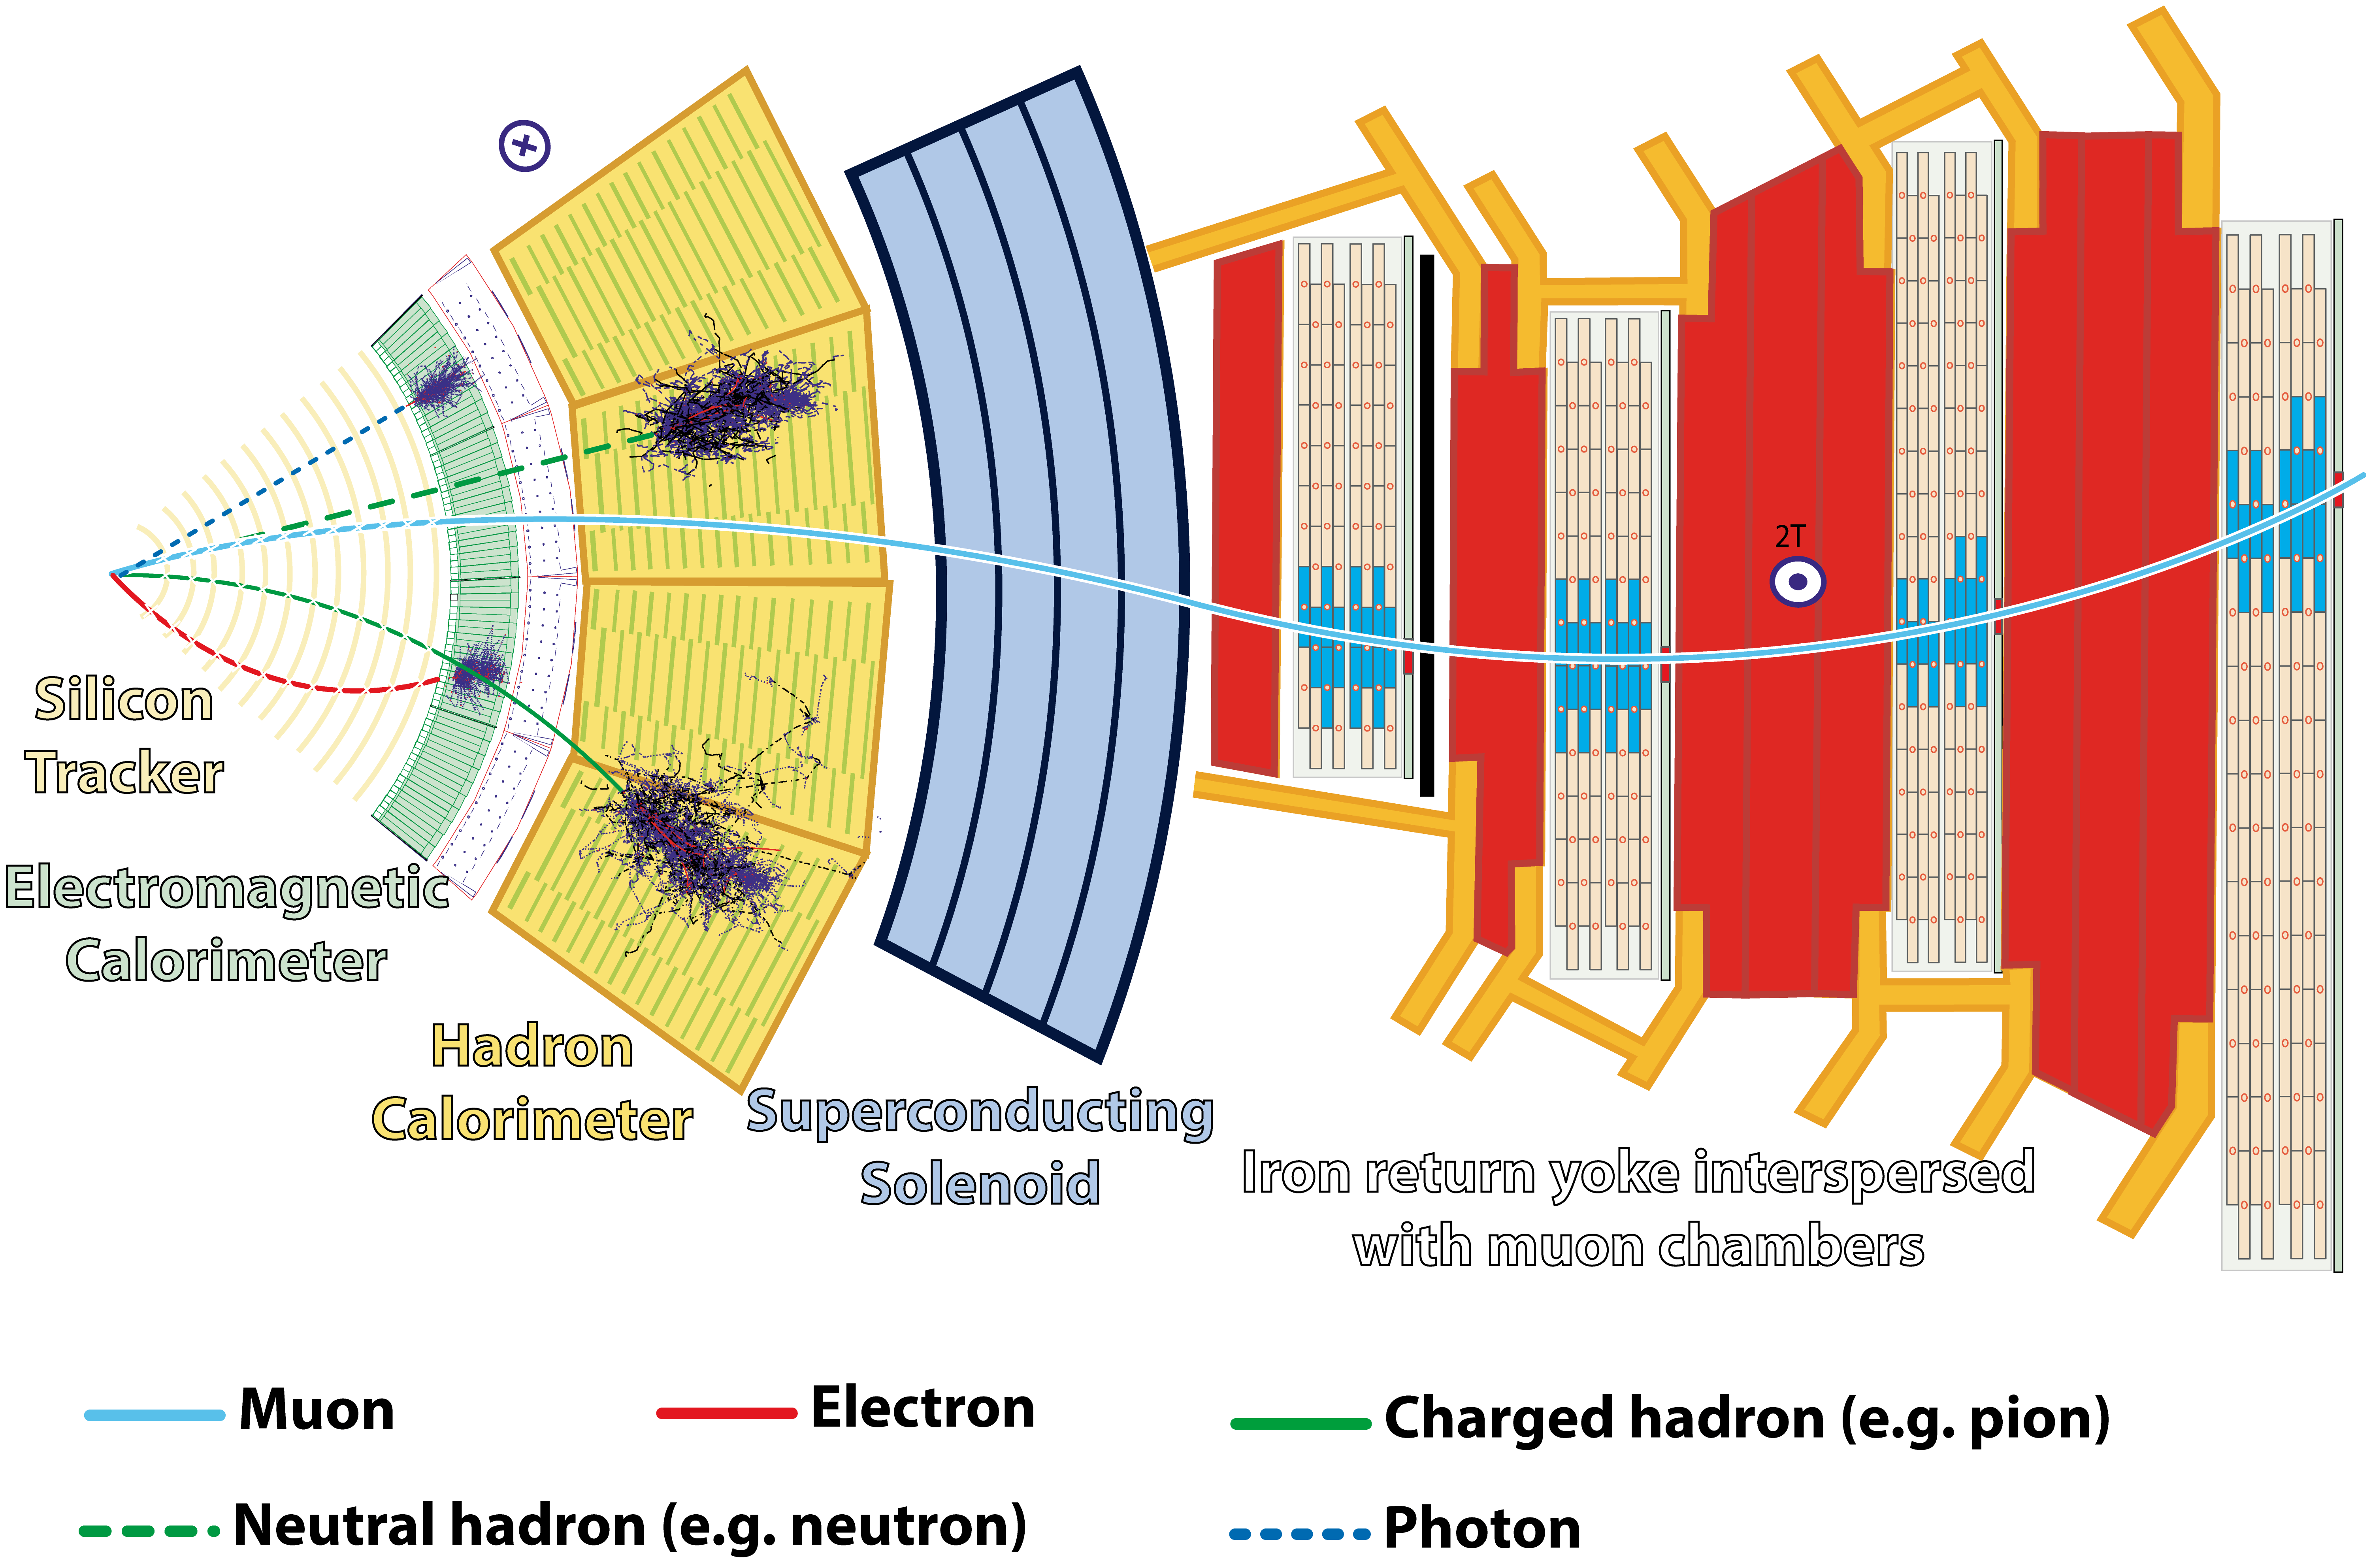
\includegraphics[width=.75\linewidth]{fig/CMS_Slice.png}
\end{center}
\caption{A section slice of the CMS detector where we can see how 
particles with different physical properties interact differently with the detector.}
\label{fig:CMS_Slice}
\end{figure}

One important kind `final-state' particles used in this thesis this charged lepton, 
which includes electrons and muons (half-life of tauon is too short);
`final-state' here means they are the end products of decay chain and interact with detector
components directly. If we concentrate on the red and blue lines in \ref{fig:CMS_Slice}, we
can see that for the electrons (red), they leave a few hits (4) that resemble a curved
track within the Silicon Tracker layer and are stopped at the Electromagnetic Calorimeter
(ECAL). 

For the muons (blue line in \ref{fig:CMS_Slice}), they largely go through all the interior layers unhinged due to their
high mass; pay close attention to the `S'-shaped curve, this is due to the opposite magnetic
field outside of the superconducting solenoid. Although information such as momentum relies on
hits on the silicon tracker, the hits in the muon chambers and a matching trajectory is needed 
for the object to be reconstructed as a muon. Notice how the
muon chambers occupy more than half of the detector by size, such design allows the CMS 
detector to excel in muon measurements and is the primary reason for the overall design.
% \todo[inline]{TODO: PF and anti-k algorithm in the context of this thesis}

Zooming out from the individual component of the CMS detector, the complete reconstruction
process is complex and sometimes requires information from multiple parts of the detector, this
algorithm is called the Particle Flow (PF) \cite{particle_flow}. While simple and neutral object like photon whose 
energy is directly measure by the ECAL (with correction for zero-suppression), electron measurements
need the information from the inner tracker (one way to determine momentum), energy at the ECAL, and
also sum of the energy of photons produced by bremsstrahlung compatible with the electron's track.

For gluons and quarks that come out of the interaction vertex, due to quark confinement, the detector 
is only be able to `see' a narrow `spray' of final state (stable) particles whose collection is called `jet'.
There are different ways and criteria to combine a collection of measurements into a single physical object,
and in CMS, the anti-$k_t$ clustering algorithm is used. In short, the algorithm would cluster objects
in a cone (meaning it has a fixed $\eta-\phi$ space) originated from the vertex according to some parameter.
But it also needs to be resilient to QCD effects that would cause jet to split, such as shown in Fig.
\ref{fig:jet_split}, where previous generation of algorithm may misidentify them.

\begin{figure}[htb]
\begin{center}
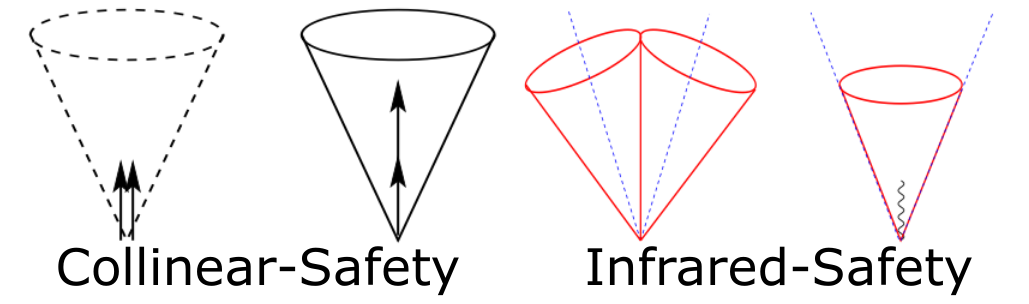
\includegraphics[width=.85\linewidth]{fig/jet_split.png}
\end{center}
\caption{A illustration of two kinds of QCD effects in jets\protect\footnotemark}
\label{fig:jet_split}
\end{figure}
\footnotetext{\url{https://twiki.cern.ch/twiki/bin/viewfile/Sandbox/Lecture?rev=1;filename=Philipp\_Schieferdeckers\_Lecture.pdf\#page=3}}

In this analysis, we use the AK4 jets which means that the algorithm is given a $R=0.4$ parameter, another
common choice is $R=0.8$ which is preferred in some cases for boosted topologies due to a larger `opening
angle'.

\section{The Higgs boson and off-shell methods}\label{sec:physics_offshell}
[1]Caola F, Melnikov K. Constraining the Higgs boson width with ZZ production at the LHC. Phys Rev D 2013;88:054024. https://doi.org/10.1103/PhysRevD.88.054024.

The importance of a Beyond the Standard Model (BSM) physics is self-evident, though the SM is one
of the most precise theory in physics we ever had, the model requires many `inputs' from experiment
for parametrization, and, it cannot account for phenomena such as neutrino oscillation with its
original form. While the direct searches in the past few years have all yield null results,
many indirect probing have been going as well.

As mentioned above, the Higgs boson has a special place as it can be seen as a `bridge' between
the SM and the BSM (in some models) as some SUSY particles can decay into it or it can decay
into SUSY particles, or simply have a BSM production Feynman diagram that leads to more Higgs
bosons than the SM would expect. In any of these cases, the basic properties of the SM Higgs
boson remain important.

Many properties are well measured, such as it's mass and spin \cite{higgs_papers}, others, however,
have not entered the realm of `precision' physics so far. One of them is the decay width of
the Higgs boson, which is of course associated to the particle's half-life. The SM predicts
that the Higgs boson to have a decay width of \SI{4.1}{\mega\electronvolt}. The problem is
that the energy resolution of the CMS detector, which is around $\mathcal{O}(1)$\si{\giga\electronvolt}
for the di-photon or 4-leptons final states, is not even remotely small enough to check this 
prediction directly.

I will give a very brief account\cite{ulascan} for the proposed (and been completed in previous years' run)
method that can constrain the Higgs decay width using events that fall into the off-shell
tail.

When the Higgs boson decays to two vector bosons (VV), in the scope of this thesis, two Z bosons,
either one of the vector bosons is off-shell, or the Higgs boson is off-shell, this is because
$m_\text{H}\approx\SI{125}{\giga\electronvolt}$ is smaller than the 
mass of two \PW{}'s($\approx\SI{160}{\giga\electronvolt}$) 
or two \PZ{}'s($\approx\SI{182}{\giga\electronvolt}$). The Higgs boson decay branching ratio
is coupled to the daughter particles' mass thus this cross section
$\sigma_{\mathrm{H}\rightarrow\mathrm{VV}}$ is enhanced as the mass of Higgs boson gets closer to 
the on-shell VV mass.  

In fact, the production of Higgs boson from a pair of vector boson is also related to the
decay width of Higgs boson $\Gamma_\text{\PH}$ via the propagator term. In terms of the
differential cross section:
\be
\label{eqn:diff_xsec}
\frac{\mathrm{d} \sigma_{\mathrm{vv} \rightarrow \mathrm{H} \rightarrow \mathrm{VV}}}{\mathrm{d} q_{\mathrm{H}}^{2}} 
\sim 
\frac{g_{\mathrm{vvH}}^{2} g_{\mathrm{HVV}}^{2}}{\left(q_{\mathrm{H}}^{2}-m_{\mathrm{H}}^{2}\right)^{2}+m_{\mathrm{H}}^{2} \Gamma_{\mathrm{H}}^{2}}
\ee
where the two $g$ on the right-hand side are the couplings for production from VV and decay
to VV respectively. Integrating this equation near the on-shell mass of the SM Higgs boson 
or in the tail region (above the mass of VV), one can translate the differential cross section
into event rate that can be (in theory) measured in experiments:
\begin{equation}
\begin{split}
&N_{\mathrm{vv} \rightarrow \mathrm{H} \rightarrow \mathrm{VV}^{*}}^{\text{on-shell}} \sim \frac{g_{\mathrm{vvH}}^{2} g_{\mathrm{HVV}}^{2}}{m_{\mathrm{H}} \Gamma_{\mathrm{H}}} \sim \mu_{\mathrm{vvH}}
\\
&N_{\mathrm{vv} \rightarrow \mathrm{H}^{*} \rightarrow \mathrm{VV}}^{\text{off-shell}} \sim \frac{g_{\mathrm{vvH}}^{2} g_{\mathrm{HVV}}^{2}}{\left(2 m_{\mathrm{V}}\right)^{2}} \sim \mu_{\mathrm{vvH}} \cdot \Gamma_{\mathrm{H}}
\end{split}
\end{equation}
The key takeaway is that, up to some correction factors, the event rates of off-shell scales
linearly respect to the Higgs decay width $\Gamma_\text{\PH}$ which allows us to indirectly
measure the width itself.

In this thesis, we will focus on the $\mathrm{H} \rightarrow \mathrm{ZZ} \rightarrow 2\ell2\nu$ channel
at the CMS detector using simulated (MC) events. This work done here is part of the ongoing work
within a group formed by UCSB HEP group, Universit\'e Libre de Bruxelles, and Beihang University under
the CMS Collaboration\footnote{Internally, CMS AN-20-081}. The analysis items and methods included in this
thesis is a subset of what will be in the official analysis and is a part of the final measurement. More
detail on what approximation has been taken in order to obtain a preliminary expected result is discussed
in the next few sections.

% \todo[inline]{maybe elaborate a bit more?}
% \newpage\phantom{blabla}


\section{Background and signal simulation}
% [1]Agostinelli S, Allison J, Amako K, Apostolakis J, Araujo H, Arce P, et al. Geant4—a simulation toolkit. Nuclear Instruments and Methods in Physics Research Section A: Accelerators, Spectrometers, Detectors and Associated Equipment 2003;506:250–303. https://doi.org/10.1016/S0168-9002(03)01368-8.

% [2]Gritsan AV, Roskes J, Sarica U, Schulze M, Xiao M, Zhou Y. New features in the JHU generator framework. ArXiv:200209888 [Hep-Ex, Physics:Hep-Ph] 2020.

% [3]The NNPDF Collaboration, Ball RD, Bertone V, Carrazza S, Deans CS, Del Debbio L, et al. Parton distributions for the LHC Run II. J High Energ Phys 2015;2015:40. https://doi.org/10.1007/JHEP04(2015)040.

% [4]Melia T, Nason P, Röntsch R, Zanderighi G. W+W-, WZ and ZZ production in the POWHEG BOX. J High Energ Phys 2011;2011:78. https://doi.org/10.1007/JHEP11(2011)078.

% ---
The following list contains the MC samples (by physical process) used in this thesis, of the first two
contain (off-shell) Higgs boson in the intermediate state:
\begin{itemize}
\item ggZZ offshell: Gluon fusion $\textsl{g}\textsl{g} \rightarrow\mathrm{H}\rightarrow\mathrm{ZZ}$
\item VVZZ offshell: Vector Boson Fusion (VBF) into Higgs
\item qqZZ, qqWZ, qqWW
\item DY: Drell-Yan process
\item TT: $t\bar{t}$, including samples with additional vector boson (TTW/TTZ) or photon + jets (TTGJets).
\end{itemize}

Various programs are used in the long chain of simulated events production.
\textsc{POWHEG BOX}\xspace\cite{POWHEG} is used for the signal simulation.
\todo[inline]{A description of LO / NLO and various program and NNPDF version etc.\ involved}

Before diving into the procedure in which the signal samples are separated generated and
subsequently combined with a re-weighting procedure, it would be appropriate to give
an account for the general idea behind the `event weight' and its significance.

As described in the beginning of this section, events correspond to different physical
processes are generated in different MC settings at different `order' of the QCD/QED physics.
Naively, one would imagine a process where the MC can directly simulate the physics at
LHC at a given center-of-mass energy. Unfortunately this is neither efficient nor possible:
not possible because some physical processes (especially QCD ones) are non perturbative and
post hoc procedures are needed to `add' physical object into the simulation. Not to mention
that the SUSY physics we are searching for does not have a `true model' known.

It is also not efficient because the processes an analysis concerns (for example, in all SUSY
searches) usually have a tiny (if not 0) cross section compare to other common ones find at
$\sqrt{\mathrm{S}} = \SI{13}{\tera\electronvolt}$ at LHC.\@ And it would be a waste of
computing resources to generate the common processes over and over.

\begin{table}[]
\centering
\begin{tabular}{|c|c|c|}
\hline
\multicolumn{3}{|c|}{Example of some important weights}                                                                                       \\ \hline
Name                  & abbr.   & Description                                                                                                 \\ \hline
Generator weight      & GEN wgt & Given by MC event generator                                                                                 \\ \hline
Pile-up weight        & PU wgt  & Correction for the pile-up effect                                                                           \\ \hline
Matrix element weight & ME wgt  & From generator that uses ME Likelihood approach \\ \hline
K-factor              & Kfactor & Correction for LO cross section of QCD processes                                                         \\ \hline
\end{tabular}
\caption{An incomplete list of weights used in the MC events used.}
\label{tab:MC_wgts}
\end{table}

In reality, Monte Carlo events are each given many `weights' (Tab. \ref{tab:MC_wgts}), so that
we don't have to generate uninteresting processes, and at the same time, for the events that lack
in number (results in poor statistics in the distribution), one can optionally generate
extension events set for it. Also, this enables the generation of `unknown' processes which can
be used to constrain possible new physics in a likelihood fit (against null hypothesis).

In this thesis, we explicitly use K-factors and scale-up and scale-down of it to 
obtain Electromagnetic systematics in qqZZ/qqWZ/qqWW backgrounds. For the signal processes involving
Higgs boson, a special treatment is given to merge and obtain high statistics sample from
multiple samples with different `true' Higgs mass. Corresponding to the $m_\mathrm{H}$ term
in the denominator on the right hand side of Eq.~\ref{eqn:diff_xsec}.
This approach is also necessary for generation of off-shell (Higgs) decays. The procedures 
and the resultant combine signal sample will be discussed in the next chapter.


\chapter{Methods}
% Methods
In this chapter, a description of event selection is given, as well as definitions of
key physical variables and how they are used to select events. Then, a procedure regarding
how the signal sample is manipulated to produce a high statistics off-shell Higgs sample is presented.
Finally, the binning of variables used to obtain the results is determined and defined.

\section{Event selection and physical variables}
Proton bunches cross each at a rate of about \SI{400}{\mega\hertz} in the beam line of
the LHC, naturally, not all of these crossings are recorded due to both technical
limitation of the electronics as well as the fact that the vast majority of these
crossings don't produce inelastic collision that is energetic enough to be interesting.

After the selection of Level 1 (L1) trigger and the higher level trigger (HLT), less than 1000
events per second are permanently recorded and would go to off-line, full reconstruction. Among these,
we only select the ones that passes certain HL triggers:
\begin{itemize}
    \item HLT\_Mu17\_TrkIsoVVL\_Mu8\_TrkIsoVVL\_DZ\_Mass3p8
    \item HLT\_IsoMu24
    \item HLT\_Ele23\_Ele12\_CaloIdL\_TrackIdL\_IsoVL
    \item HLT\_DoubleEle25\_CaloIdL\_MW
    \item HLT\_DoublePhoton70
    \item HLT\_Ele32\_WPTight\_Gsf
    \item HLT\_Photon200
\end{itemize}
Most of the trigger names are self-explanatory, and are the starting point of the analysis. The
purpose of the triggers is to insure events in the corresponding samples would contain the physics
we wanted (since run data samples are divided according to what triggers they passed).

The next step is to `add' composite variables that is significant to the physics of interests as
well as making base-line cuts on the events.
The jets are all AK4 jets unless mentioned otherwise, and a special type of jets, called B-tagged
jets are produced using DeepFlavour algorithm.\cite{btag} We shall also define a few of the
uncommon variables in the list, and physical motivations are given in the following
paragraphs.

After mandating passage of the set of triggers above, based on more delicate physics reasons, 
the baseline cuts are:
\begin{itemize}
    \item No ak4-jet b-tagged jet
    \item Both leptons have $p_\mathrm{T} > \SI{25}{\giga\electronvolt}$
    \item $\abs{\Delta\phi_{\ell\ell\_\met}} > 1.0$
    \item $\abs{\Delta\phi_{\ell\ell\mathrm{Jets}\_\met}} > 2.5$
    \item $\abs{m_{\ell\ell} - 91.2\gev} < 15\gev$:
        the signal process consists of $\mathrm{Z}\rightarrow{}\ell\ell$, we
        require the di-lepton system has a mass that is consistent within the Z mass peak.
    \item $p_\mathrm{T}^{\ell\ell} > 55\gev$: 
        the Drell–Yan (DY) process creates a lot of backgrounds events, but their di-leptons
        go back-to-back with expected value of this variable close to 0.
    \item $\met > 125\gev$:
        the signal process creates true $\met$ with neutrinos, this cut also reduce bkg such
        as DY.
    \item $\min{\abs{ \Delta\phi_{\mathrm{j}\_\met}}} > 0.25$
\end{itemize}
In addition, to reduce the detector effects at high pseudo rapidity angels:
\begin{itemize}
    \item $\eta_\mu< 2.4$
    \item $\eta_e< 2.5$
\end{itemize}

A lot of the cuts are related to angles between various physical objects presented in the
reconstruction. The reason is simple: the signal events, where Higgs goes to ZZ and one Z
goes to 2 charged leptons and the other goes to 2 neutrinos, ideally would have the two Z's 
`back-to-back' in Higgs boson's rest frame, leading to a large angel in the transverse plane.
% ( assuming the $\met$ mainly comes from the two neutrinos, of course)

Furthermore, in background events which do not contain this kinematic feature, the
correlation in the directions of $\met$ and the transverse momentum of the leptons is weaker.

To use this kinematic feature to increase signal to background ratio, we define 
$\abs{\Delta\phi_{\ell\ell\_\met}}$ as the azimuthal angel (perpendicular to 
the beam line) between the di-lepton system and the transverse missing energy. In the
signal events that produce 0 jet, this variable should be $\pi$. The cut is lowered to $1.0$ 
due to the finding that in the (not so rare) cases where there are jet(s) recoiling against
the ZZ system, this variable can go quite low.

This leads to the next variable on the list, $\abs{\Delta\phi_{\ell\ell\mathrm{Jets}\_\met}}$, which
is almost the same except that we add all jets' momentum into the di-lepton system to account
for the events that have produced jets, which in turn would cause the angel be lower in
a multi-body final state.

Finally, $\min{\abs{ \Delta\phi_{\mathrm{j}\_\met}}}$ is the minimum azimuthal angel difference between
any of the jet (that passes cuts) and the $\met$, it exist because jets are one of the 
most difficult physical objects measure, they often create so-called instrumental $\met$ due to jet
mis-measurements and it can be quite large in magnitude. However, such mis-measurements often yield large
$\met$ in the direction of the original jet. This cuts requires angular separation since in signal process,
the jet recoils against ZZ system.

We also define variables that are not cut on, but are used for fitting:
\be
D_{j j}^{V B F}=\frac{P_{S M}^{V B F}(\vec{\Omega})}{P_{S M}^{g g}(\vec{\Omega})+P_{S M}^{V B F}(\vec{\Omega})}
\ee
As introduced in \cite{hig-18-002}. In short, this variable (discriminator) is sensitive
to the VBF physics and the correlation between (angels and mass of) the outgoing jets resulted from the
VBF topology. At the same time:
\be
\mtzz={\left[\sqrt{p_{\mathrm{T}, \ell\ell}^2+m_{2 \ell}^2}+\sqrt{E_{\mathrm{T}}^{\mathrm{miss}^2}+m_\mathrm{Z}^2}\right]}^2-\left[\vec{p}_{\ell\ell}+\vec{E}_{\mathrm{T}}^{\mathrm{miss}}\right]^{2}
\ee
is defined based on the hypothesis that the $\met$ is comprised of mainly the two neutrinos
from one of the Z bosons. We shall see the usefulness of this variable in channels where
not enough jets are present to construct the DJJVBF variable.

On top of the cuts stated in the beginning, several $\met$ filter and lepton isolated tracks veto
are present in the underlying analysis framework to reject events with pathological reconstruction.
% \missingfigure{Show how much backgrounds are gone for maybe 2 samples}

\section{Signal samples re-weighting}
\label{sec:sig_rewgt}
% \begin{itemize}
%     \item Physics of Higgs signal sample (the weight, ME)
%     \item the need for pieceing together samples with different LHE Mass
%     \item results (also see appendix A)
% \end{itemize}
Extra attention was given to the off-shell Higgs sample used in this thesis and two different kinds
of re-weighting of the simulated events are applied in to produced a MC sample with wide
mass spectrum way beyond the mass of Higgs ($\approx \SI{125}{\giga\electronvolt}$). We use the
gluon fusion Higgs (ggH) sample to illustrate the procedures, the same procedures are applied to
the VBF samples as well.

We start by generating separate samples with different Higgs mass (LHECandMass).
This is the mass of Higgs terms appears in the propagator on 
the R.H.S of Eq.~\ref{eqn:diff_xsec} as mentioned before. The raw distribution of the true mass
in different samples (without any weight) is shown in Fig.~\ref{fig:LHE_raw} (left). As expected, 
the peak of the distribution moves to the right as the mass of the sample becomes larger, at the
same time, the `peak' of samples with very large mass are wider because the lower edge
of the peak is dominated by an underlying exponential `tail'. We also see that for some lower mass
samples (200, 300, 400 etc.), they have a cut-off beyond $\mathrm{M}\approx2500$ which means they have 0
statistics beyond that mass range. After applying the GEN, PU, and ME weights given by their
individual MC process and JHUGen MELA, as shown in Fig.~\ref{fig:LHE_raw},
we see that they are consistent with each others' line shape. However, it is clear
that:
\begin{enumerate}[label=(\roman*)]
    \item Lower mass samples have cut-offs in the tail region
    \item Samples have poor statistics in mass windows that are 
        far from their true mass (as listed in the legend).
\end{enumerate}
The second point is best illustrated by the wide spikes of lower mass samples near their cut-offs,
as well as the visible fluctuations of high-mass samples in the mass region (don't be fooled by the 
visual, the plot is in semi-log scale).
\begin{figure}[htb]
    \begin{center}
        \subfloat[]{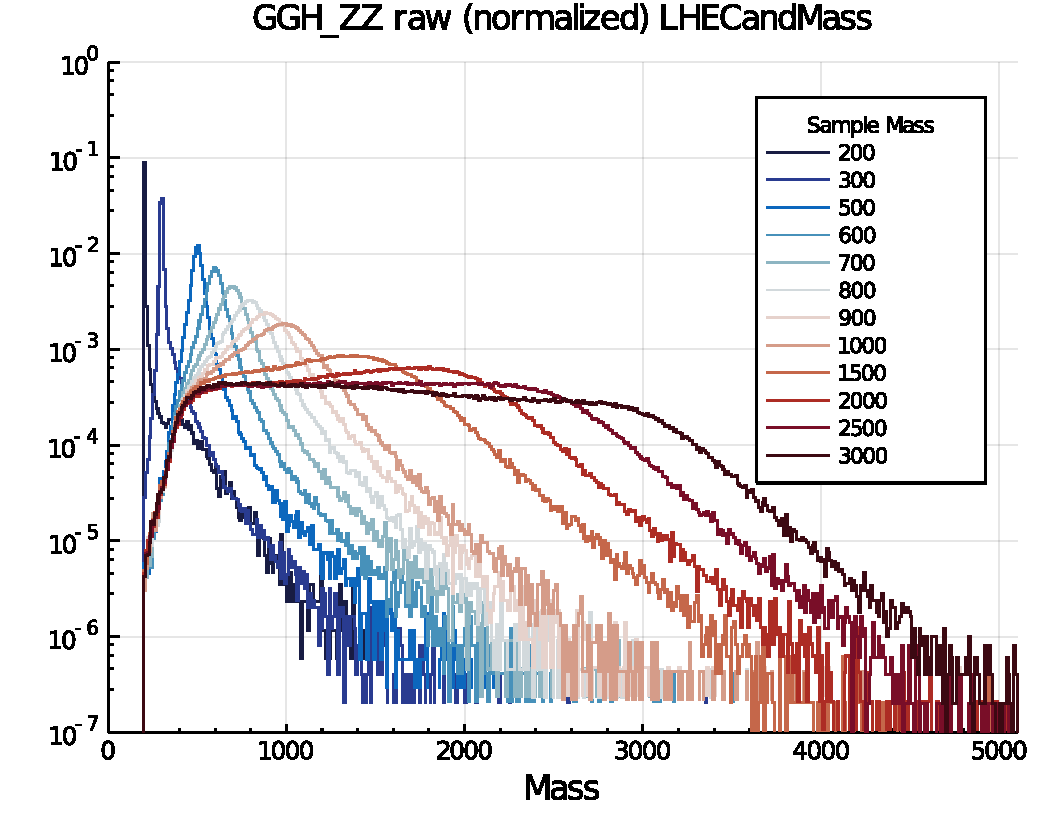
\includegraphics[width=.5\linewidth]{fig/LHE_Raw.pdf}}
        \subfloat[]{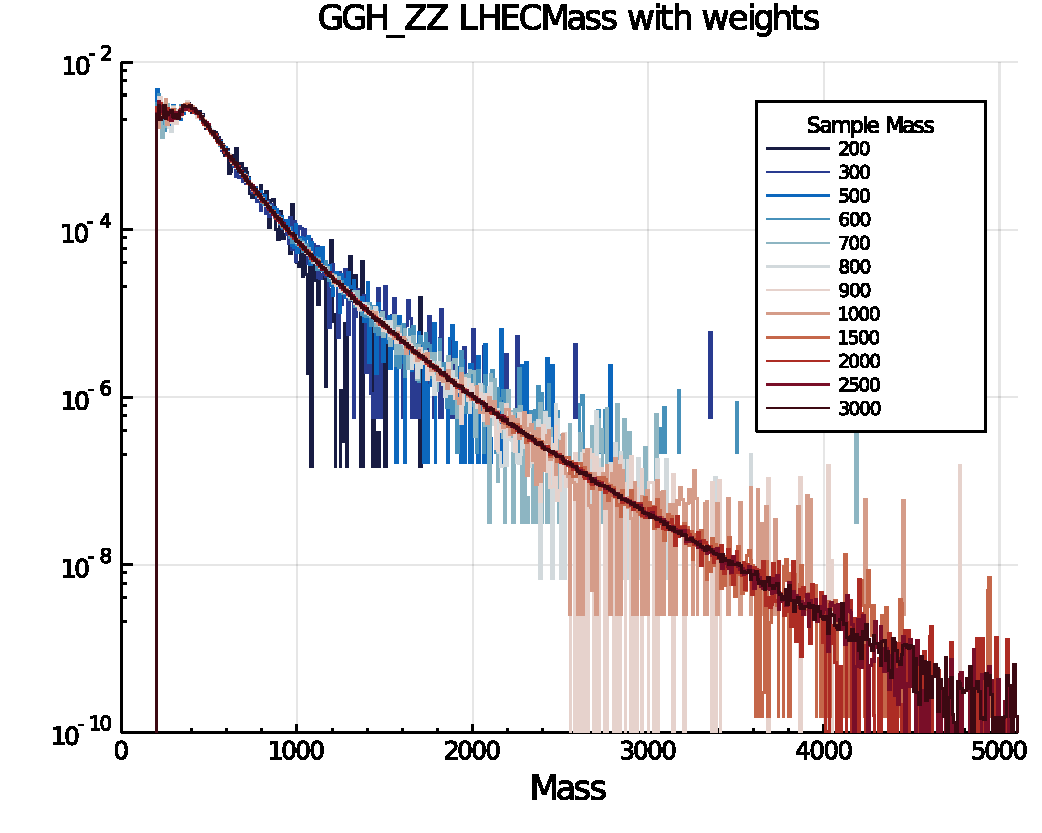
\includegraphics[width=.5\linewidth]{fig/LHE_PUME_wgts.pdf}}\\
    \end{center}
    \caption{Normalized distributions of LHECandMass before (left) and after (right) applying
        the weights. Together they show a need to combine samples for a wide-range, high
    statistics signal sample. Bin size = \SI{10}{\giga\electronvolt}.}
    \label{fig:LHE_raw}
\end{figure}

The goal of the combination of samples is to use all the events, but with a correction weight
such that each sample has a higher weight in the region where they posess good statistics. Of
course while keeping the overall normalization stays unchanged. To do this, we pick a list of
`mass windows' with edges sitting on the true masses of the samples, and we define effective
number of events $\mathrm{N}_\mathrm{eff} = \frac{(\sum\mathrm{wgts})^2}{\sum(\mathrm{wgts}^2)}$
within each mass window. Here, the wgts corresponds to the product of PU wgt, GEN wgt, K-factor, and ME weight for
the GGH sample in consideration. For a specific GGH sample $i_0$ and its events fall in a mass 
window $j$, $\mathrm{N}_\mathrm{eff}^{i_0j}$ is first obtained and a re-weighting factor can be computed:
\be
\mathrm{wgt}_\mathrm{window}^{i_0j} = 
\frac{\mathrm{N}_\mathrm{eff}^{i_0j}}{\sum_i\mathrm{N}_\mathrm{eff}^{ij}}
\ee
This factor is applied to all events from sample $i_0$ within the window $j$. Conceptually,
the effective number of events ensures the weight is not skewed by the difference in the overall
normalization of samples, and in each of the mass windows, samples with more concentrated
statistics in that window are given a higher weight. In Fig.~\ref{fig:window_wgt_matrix} (a), a
clear diagonal pattern can be seen, physically it means that samples with higher true 
mass are given a higher weight in tail mass windows--- consistent with the expected outcome.
\begin{figure}[htb]
    \begin{center}
        \subfloat[]{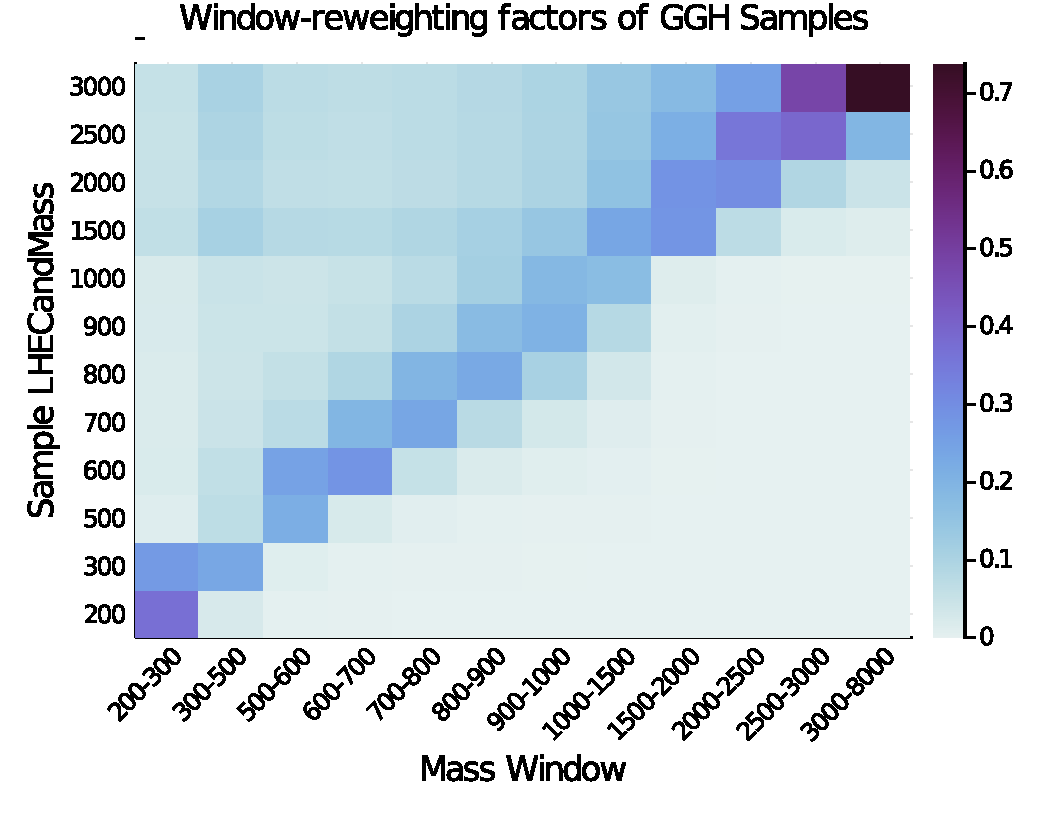
\includegraphics[width=.5\linewidth]{fig/Window_wgt_GGH.pdf}}
        \subfloat[]{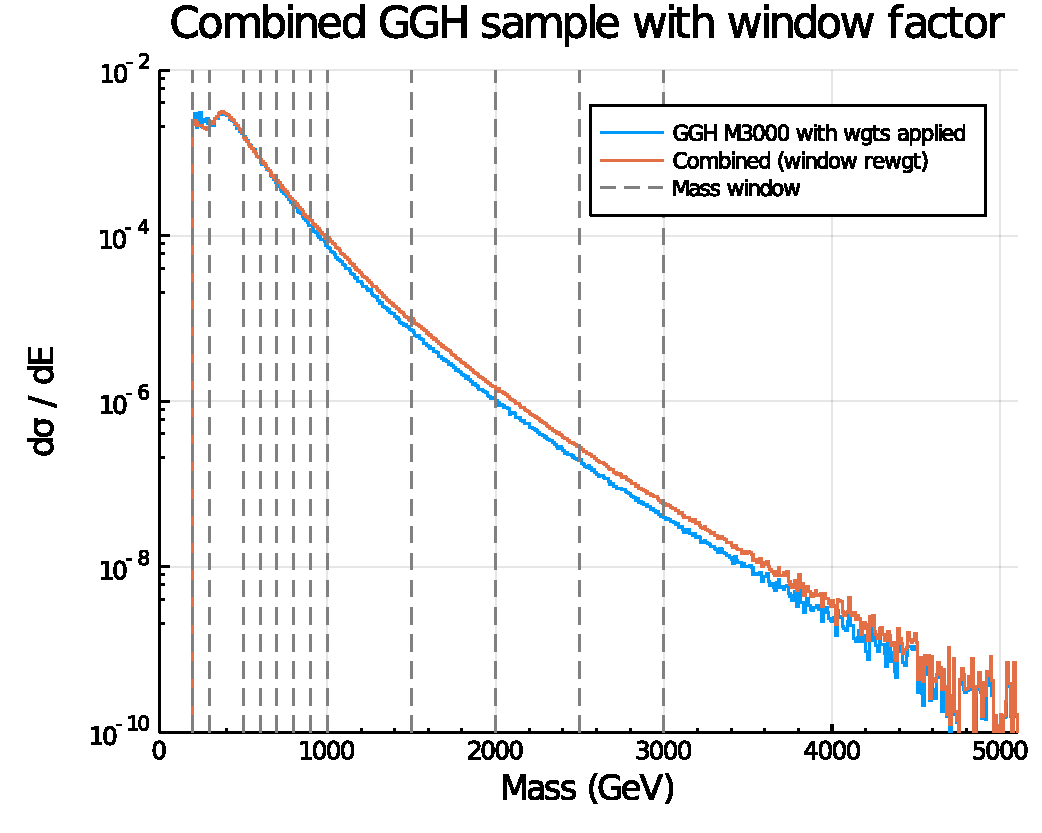
\includegraphics[width=.5\linewidth]{fig/LHC_compare_windowwgt.pdf}}
    \end{center}
    \caption{Heatmap of window re-weight factors of different samples and mass windows (left);
    effects of applying window factors for the combined sample(right)}
    \label{fig:window_wgt_matrix}
\end{figure}

However, even with the unit normalization, there are still inconsistency in the shape as shown
in Fig.~\ref{fig:window_wgt_matrix} (b). This is likely because the finite number of events
and non-infinitesimal mass window size used. We introduce another correction factor for
this small artifacts. Iteratively going through every sample, between the previous and the
next one, derive a sample mass factor based on:
\be
\mathrm{wgt}_\mathrm{mass}^{i, i+1} = \frac{\sum{\mathrm{wgt}_\mathrm{i}}}{\sum{\mathrm{wgt}_\mathrm{i+1}}}
\text{, for events that has Mass between sample mass of $i$ and $i+1$}
\ee

\begin{figure}[htb]
    \begin{center}
        \subfloat[]{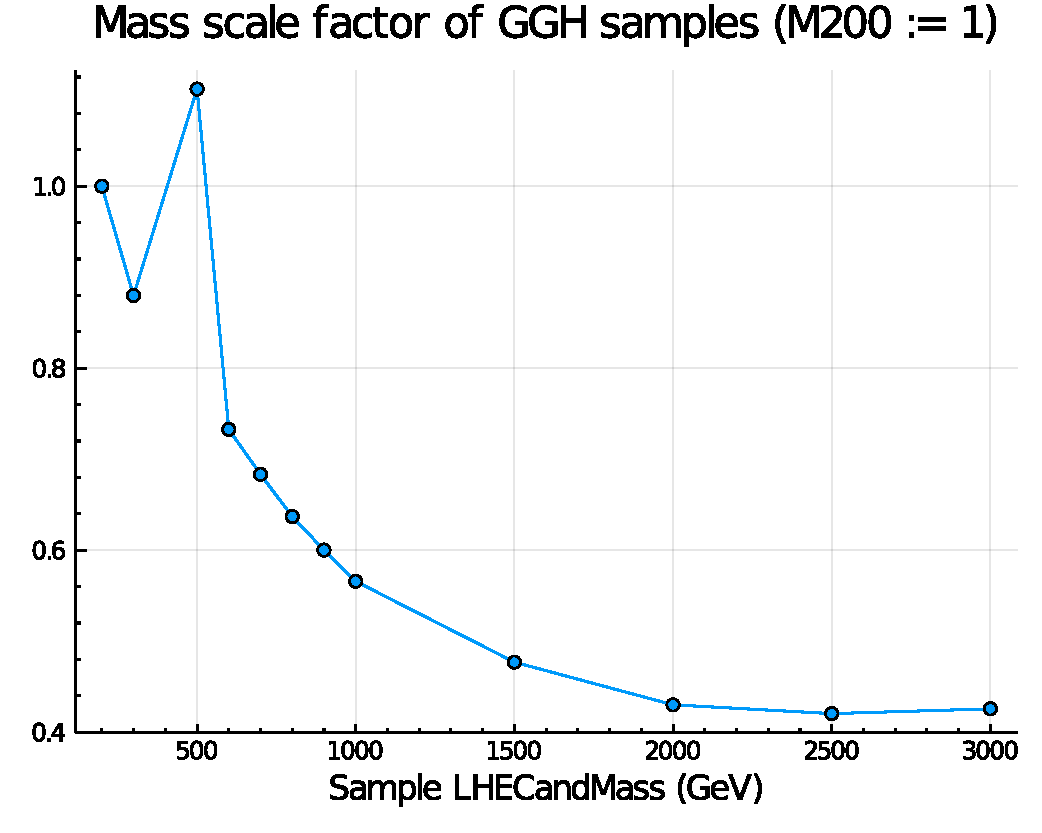
\includegraphics[width=.5\linewidth]{fig/Mass_wgt_GGH.pdf}}
        \subfloat[]{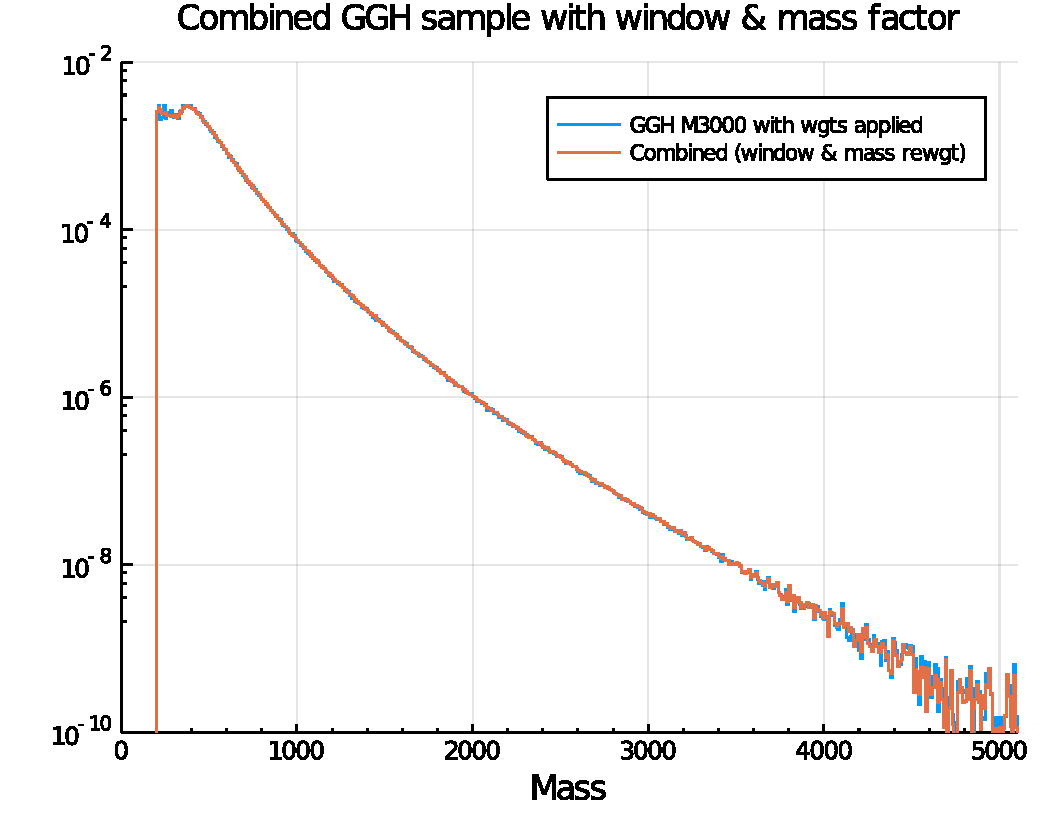
\includegraphics[width=.5\linewidth]{fig/LHC_compare_bothwgt.pdf}}
    \end{center}
    \caption{Iterative sample mass factors obtained (left) and the final combined sample (right)}
    \label{fig:LHE_rewgt}
\end{figure}

This factor corrects the high variations of overall normalizations between samples, the factors and result
are shown in Fig.~\ref{fig:LHE_rewgt}. As expected, high mass samples need a down correction (not by a lot)
to eliminate the deviated trend before.

Finally, 1.098946 is multiplied to the weights of all ggZZ processes (all of BKG, SIG, BSI
of GGH sample) as a K factor for Next-to-next-to-leading-order (NNLO) $\rightarrow$ 
Next-to-next-to-next-to-leading-order (N3LO).

Although we used the particular matrix element weights for one of the signal hypothesis, these two
correction factors apply too all hypothesis and a plot of them without normalization are shown
in Fig.~\ref{fig:bsi_sig_bkg_compare}. As expected, background exceeds signal by more than 100\%
which is partially why the constrain is hard to obtain.
\begin{figure}[htb]
    \begin{center}
        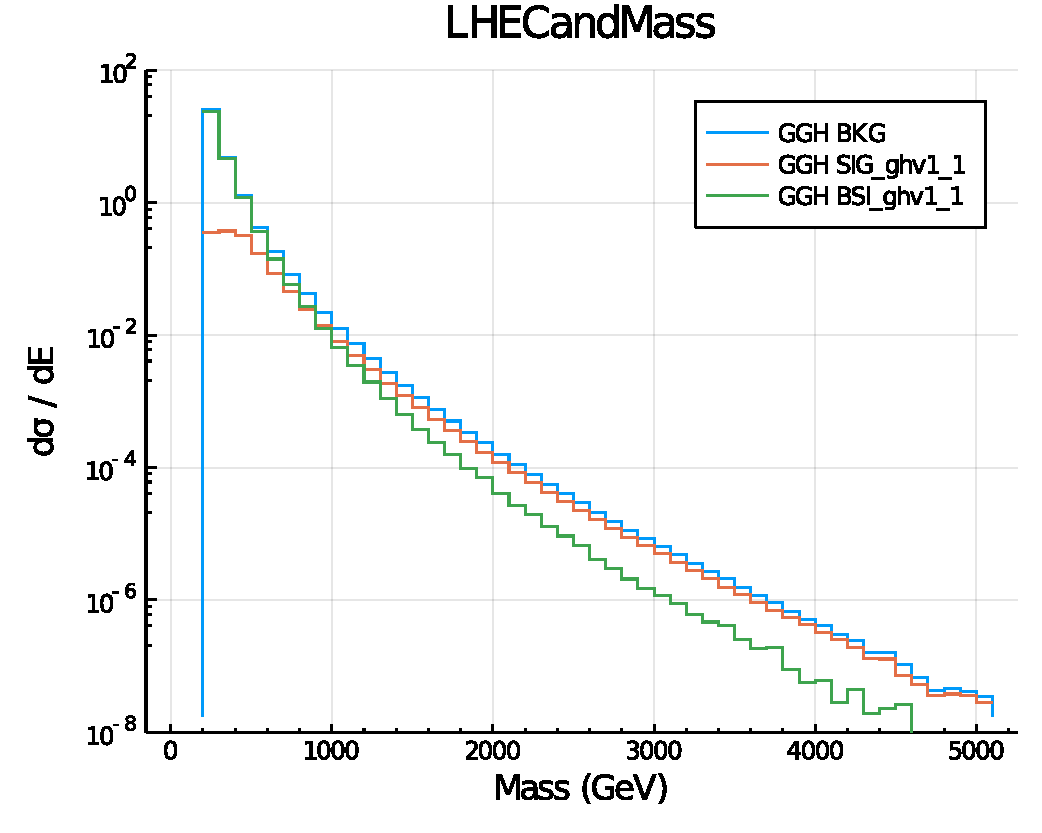
\includegraphics[width=.7\linewidth]{fig/LHE_integral_difference.pdf}
    \end{center}
    \caption{Distributions of background, signal, and background signal interaction}
    \label{fig:bsi_sig_bkg_compare}
\end{figure}

\section{Strategy in variable selection and binning and systematical uncertainties}
After preparing the signal samples and decided on the event selection criteria, we move on to
decide on the variables and their (2D histogram, as shown in Fig.~\ref{fig:templates_demo}) `binning' before a combined-limits
fit can be applied. As discussed in earlier sections, one of the more inventive variables
newly introduced specifically for the analysis is the DJJVBF discriminator. However, it is
clear that this variable is undefined for events with $\njets < 2$. To
not `waste' any statistical significance, we use $\met$ in its place for the
$\njets = 0,1$ categories. In total, we have 2 ($ee$ or $\mu\mu$) $\times$ 4 ($\njets = 0,1,2,3+$) = 8
channels to consider when making histogram templates.
Bin edges for different categories in number of jets are as the following:
\begin{itemize} 
    \item $\njets < 2$
        \begin{itemize} 
            \item $\mtzz$ = 150, 300, 400, 600, 800, 1000, 13000
            \item KD1 = DJJVBF = 0, 0.2, 0.4, 0.6, 0.8, 1
        \end{itemize}
    \item $\njets >= 2$
        \begin{itemize} 
            \item $\mtzz$ = 150, 300, 400, 600, 800, 1000, 13000
            \item KD1 = $\met$ = 125, 200, 280, 420, 500, 800, 13000
        \end{itemize}
\end{itemize}
The higher mass ($\mtzz$) bins are wider because samples
have difficulty filling them due to physical reasons (especially for backgrounds) 
and the cuts being applied. As shown in Fig.~\ref{fig:templates_demo}, the relative error (err/counts) of each
bin in the histogram templates are displayed, a balance between significance and uncertainty is
obtained. We use the above binning for all samples and 8 channels that are considered in this
thesis. See Appendix~\ref{apdx:templates_hist} for a compilation of template histograms of GGH sample.

For low-yield background samples, due to the nature of NLO samples, bins sometimes would have negative
content. To mitigate it's effect on the likelihood fitting (pathological), we replace the bin content
by (Integral of the histogram) $\times \num{e-5}$.
\begin{figure}[htb]
    \begin{center}
        \subfloat[]{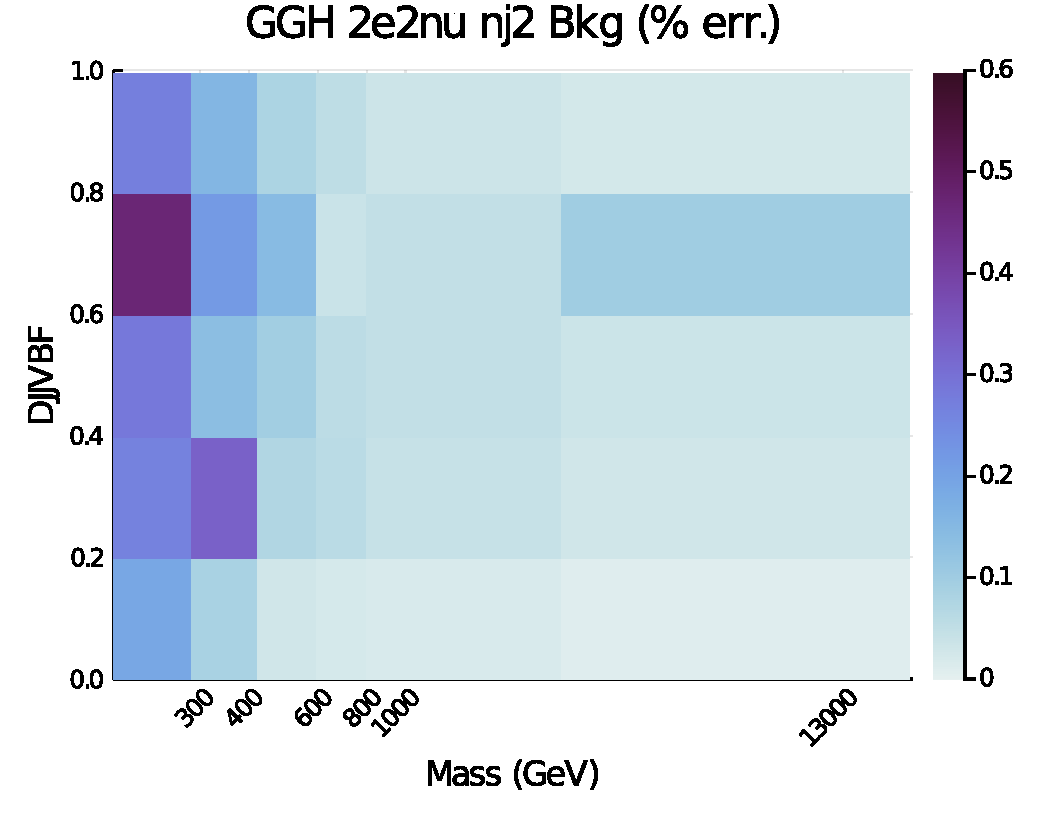
\includegraphics[width=.5\linewidth]{fig/ggZZ_templates/ggZZ_2e2nu_nj2_Bkg.pdf}}
        \subfloat[]{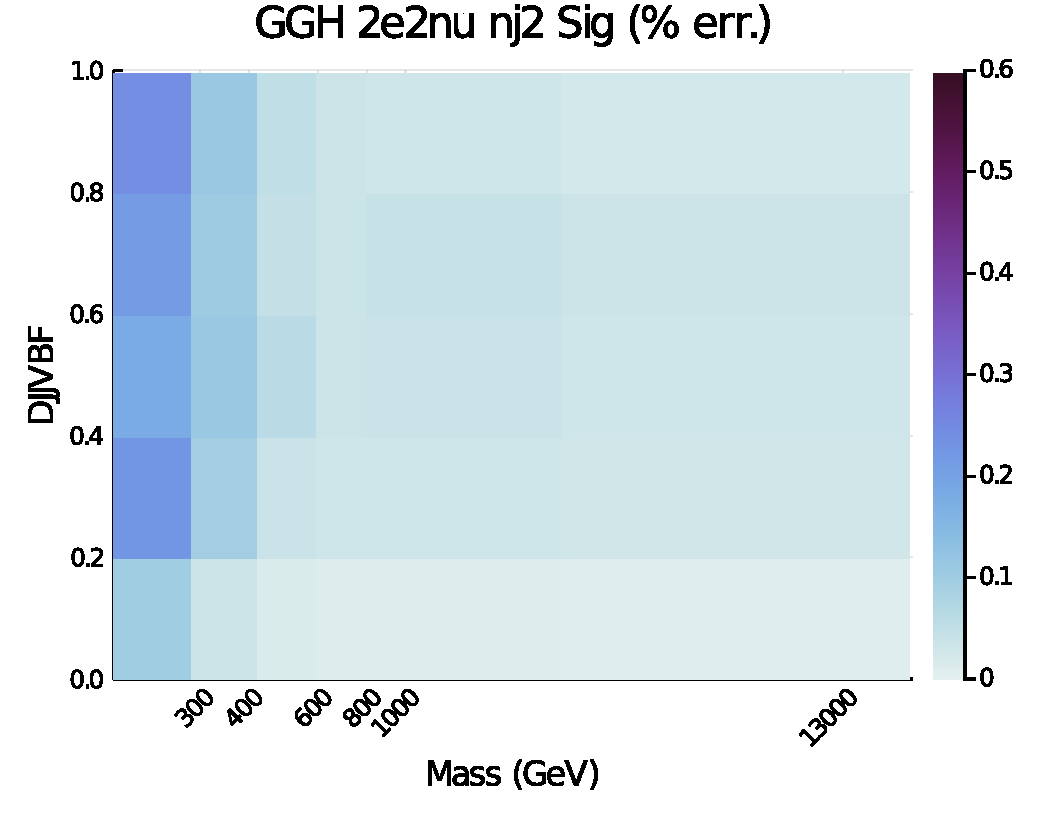
\includegraphics[width=.5\linewidth]{fig/ggZZ_templates/ggZZ_2e2nu_nj2_Sig.pdf}}
    \end{center}
    \caption{Background (left) and Signal (right) histogram templates for $2e2\nu$ with $\njets = 2$.}
    \label{fig:templates_demo}
\end{figure}

Systematical uncertainties are also included in the fitting:
\begin{itemize}
    \item Luminosoty: GGH\_ZZ, VBF\_ZZ, qqZZ, qqWZ
    \item NRB Estimation: TT
    \item Branching Ratio of Higgs to ZZ to 4l: GGH\_ZZ, VBF\_ZZ
    \item K-fatcor of backgroun gluongluon parameter
\end{itemize}
Most of them are assigned with a $ln(N)$ uncertainty of 1-$\sigma$ or 10\% except the k-factor
which is a parameters directly multiplied with backgrounds Parton Distrubution Function (PDF).


\chapter{Results and interpretation}
Final results of this thesis are presented. As the result acts as
`expected' limits, the ongoing work and potential interpretation are discussed.
\pagebreak
% TODO
% 1) where it intersects -2deltaNLL=3.84
% 2) what is the value of -2deltaNLL at muoffshell=0
\section{Limits on Higgs decay width}
\begin{figure}[htb]
    \centering
    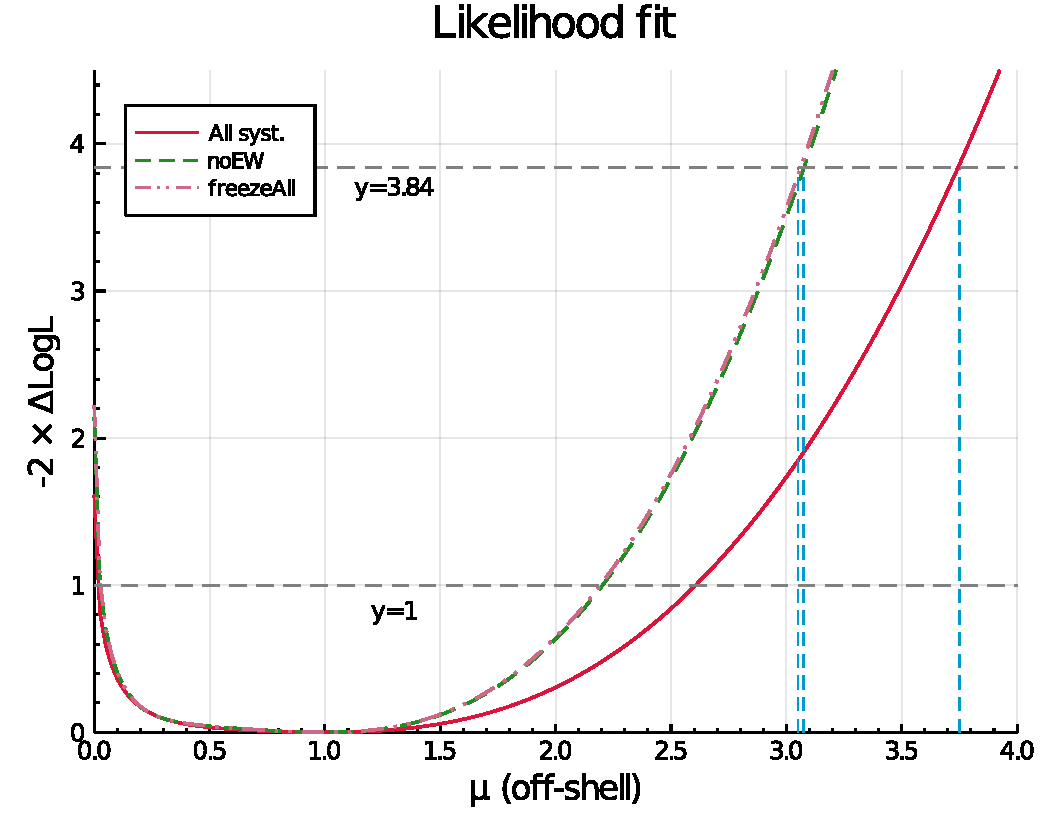
\includegraphics[width=.8\linewidth]{fig/Final_fit_mu_offshell.pdf}
    \caption{Maximum likelihood fit of $\mu^\mathrm{H}_\mathrm{off-shell}$ (off-shell rate ratio).
    For all systematics (red), no Electroweak syst.~(green),
    0 syst.~(orange): y-intersect=\{1.61, 2.14, 2.22\}, 1$\sigma$ lower limits=\{0.025, 0.025, 0.025\},
1$\sigma$ higher limits=\{2.6, 2.2, 2.2\}, 95\% CL limits=\{3.75, 3.08, 3.05\}, respectively.}
    \label{fig:final_fit_mu}
\end{figure}
After running through Combined Limited tool~\cite{combine1, combine2, combine3} for likelihood fitting, we first extract the significance
of the off-shell rate.~(Fig.~\ref{fig:final_fit_mu})
The y-axis is understood to be $\sigma^2$ in terms of significance, thus
the intersection with the y-axis is the signal sensitivity, or in other words,
rejection of the 0 width hypothesis (no off-shell), which has a significance of 
$\sqrt{1.61} \approx 1.26\sigma$ in this fit with all the systematic uncertainties included.
As the systematics are turned off', the constraint becomes tighter, producing an error band for the expected
final result in the upcoming official analysis. The electroweak uncertainty is displayed individually as
it encompass most of the systematic uncertainties.

\begin{figure}[h]
    \centering
    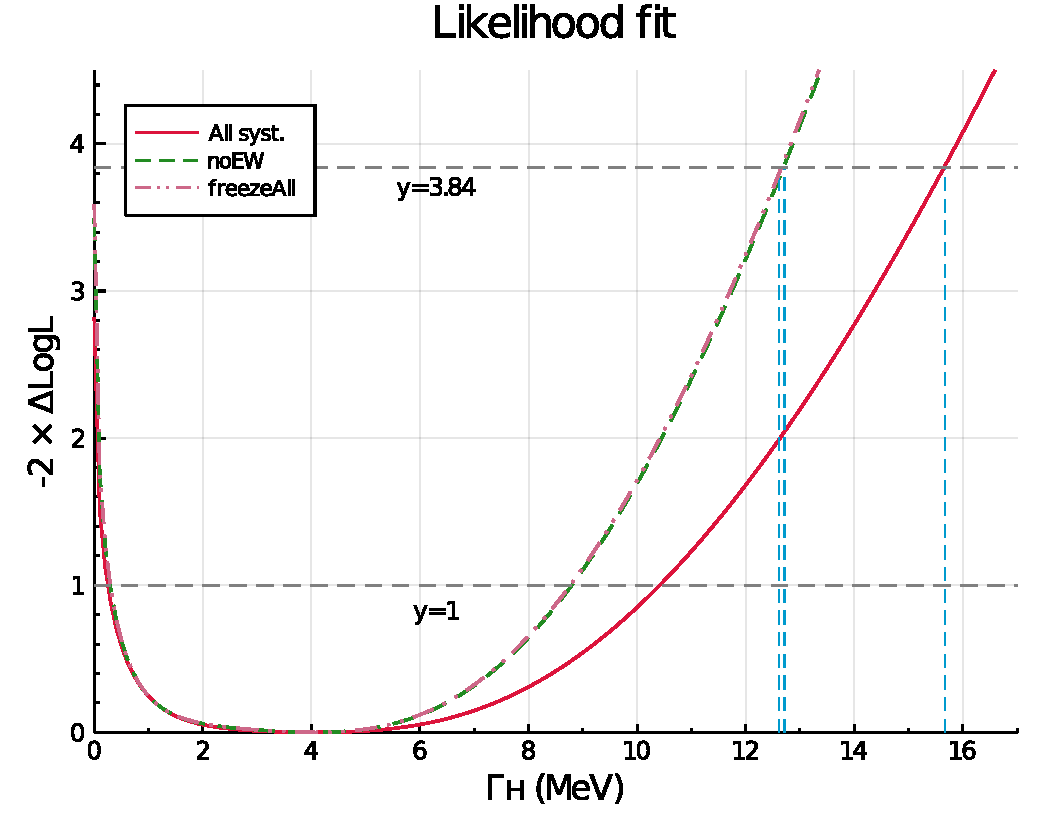
\includegraphics[width=.8\linewidth]{fig/Final_fit_width.pdf}
    \caption{Maximum likelihood fit of Higgs decay width. For all systematics (red), no Electroweak syst.~(green),
    0 syst.~(orange): y-intersect=\{1.61, 2.14, 2.22\}, 1$\sigma$ lower limits=\{0.10, 0.10, 0.10\} MeV,
1$\sigma$ higher limits=\{10.78, 9.16, 9.06\} MeV, 95\% CL limits=\{16.38, 13.33, 13.23\} MeV, respectively.}
\label{fig:final_fit_width}
\end{figure}
Furthermore, by un-constraining the $\mu_\mathrm{F}$ and $\mu_\mathrm{V}$ which are the production rate
of Higgs from fermion fusion vs.\ massive boson fusion, as mentioned in the Eqn.~\ref{eqn:diff_xsec}.
We adopt the range suggested~\cite{rfrv_higgs_pas}. The constraint on the decay width of Higgs $\Gamma_\mathrm{H}$ is shown in 
Fig.~\ref{fig:final_fit_width}. The minimal (max likelihood) falls on \SI{4.07}{\mega\electronvolt},
consistent with the Standard Model hypothesis being used. 
Again, 1$\sigma$ and 95\% CL are marked respectively. And a final result of 
$\Gamma_\mathrm{H}<\SI{16.38}{\mega\electronvolt}$ can be quoted.




% without that, what you are showing is actually off-shell signal strength with the assumption that the ratio 
% of the signal strengths for gg and EW productions are as in the SM.


\appendix
\chapter{Weights Table for Higgs Sample}

\chapter{Additional Figures}
\pagebreak
\section{GGH Sample Fitting Templates of Background and Signal}
\label{apdx:templates_hist}
\begin{figure}[hbt]
\begin{center}
\subfloat[]{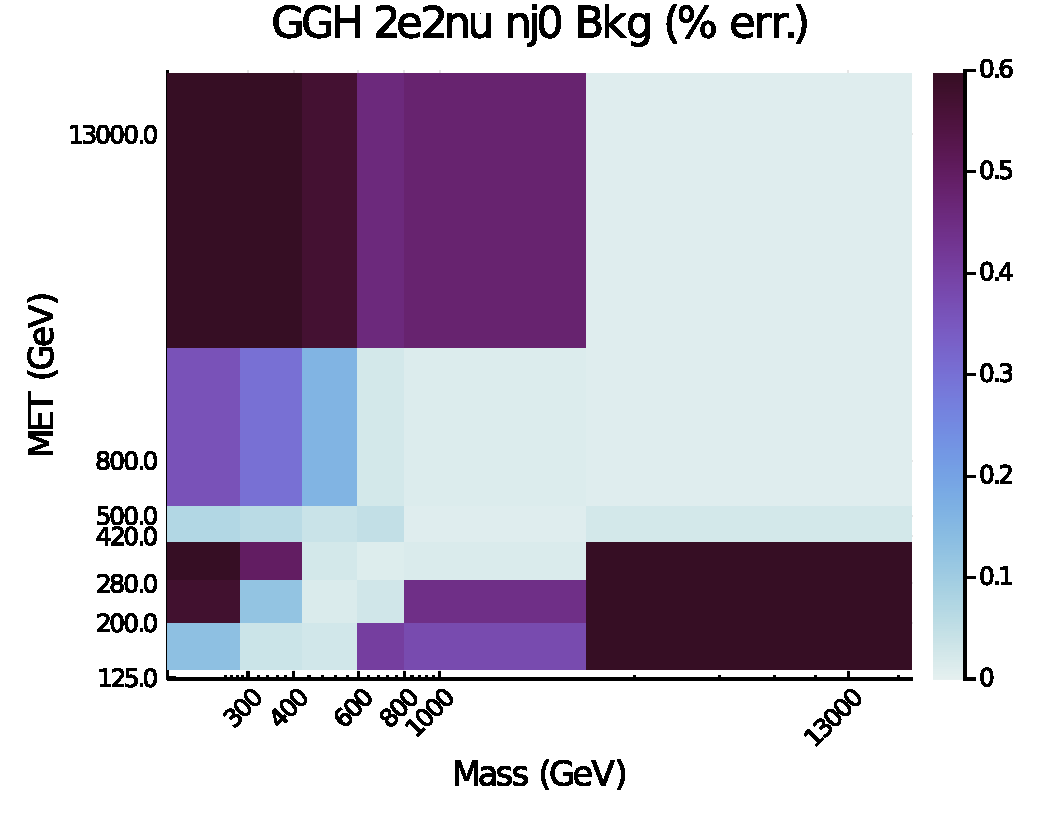
\includegraphics[width=.33\linewidth]{fig/ggZZ_templates/ggZZ_2e2nu_nj0_Bkg.pdf}}
\subfloat[]{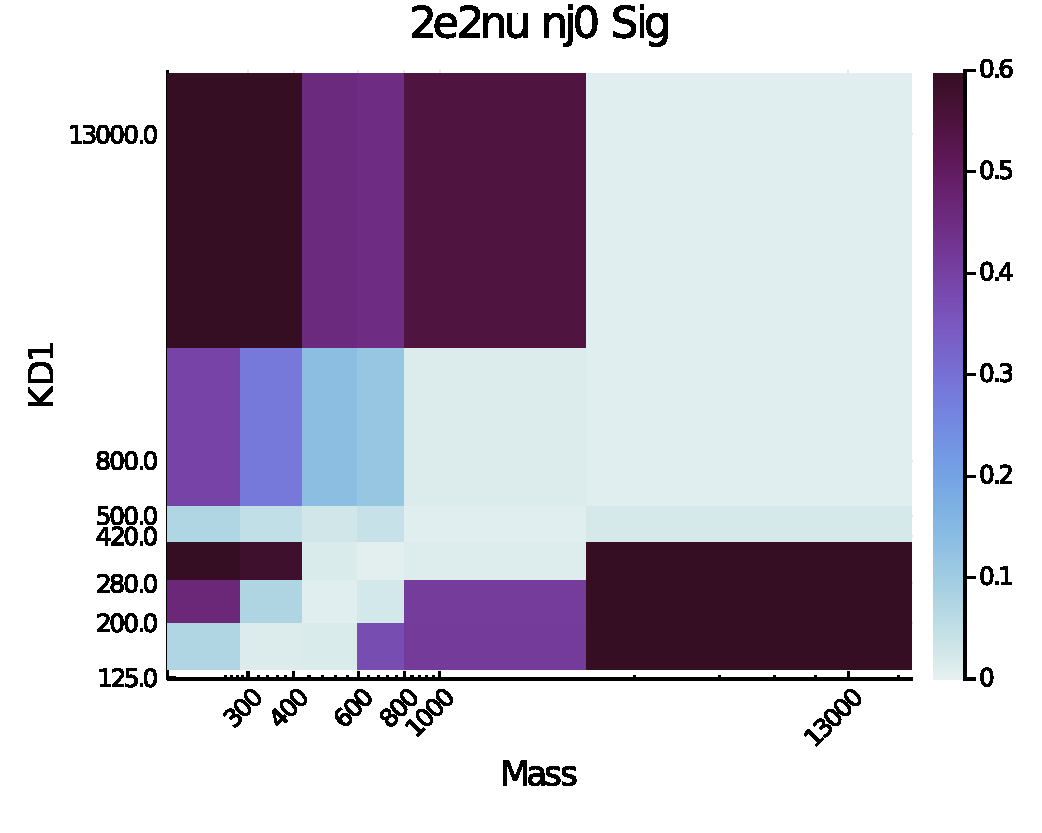
\includegraphics[width=.33\linewidth]{fig/ggZZ_templates/ggZZ_2e2nu_nj0_Sig.pdf}}
\subfloat[]{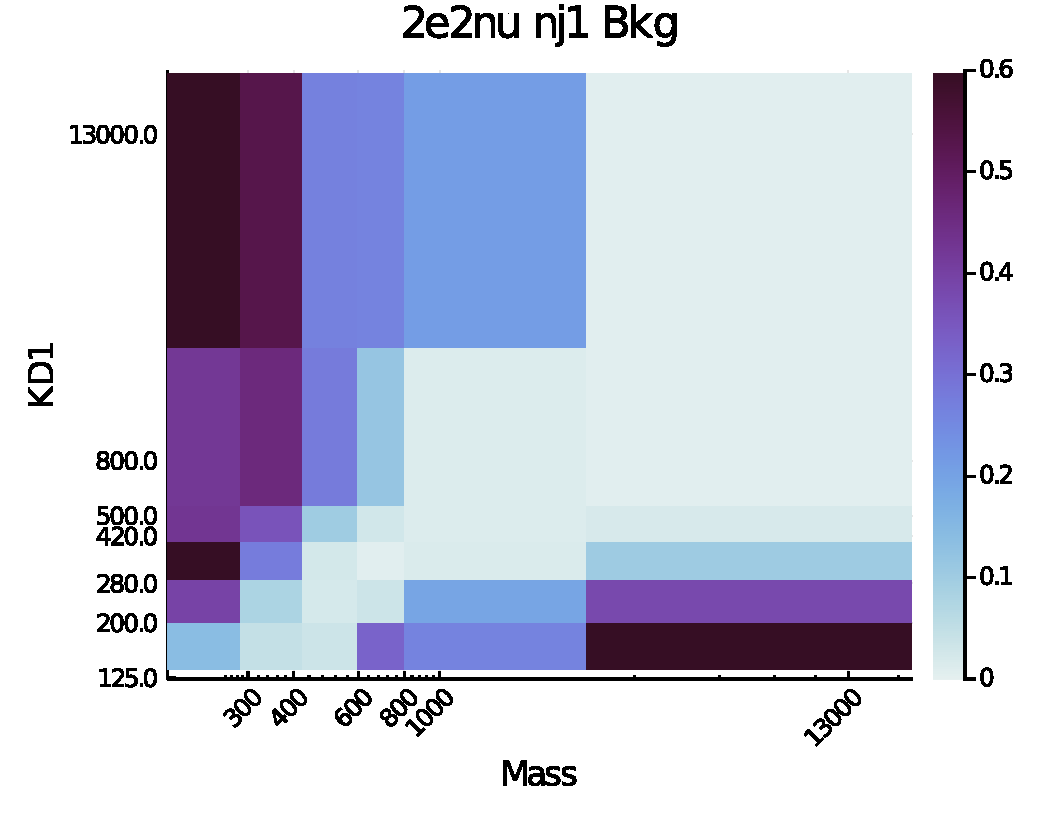
\includegraphics[width=.33\linewidth]{fig/ggZZ_templates/ggZZ_2e2nu_nj1_Bkg.pdf}}\\
\subfloat[]{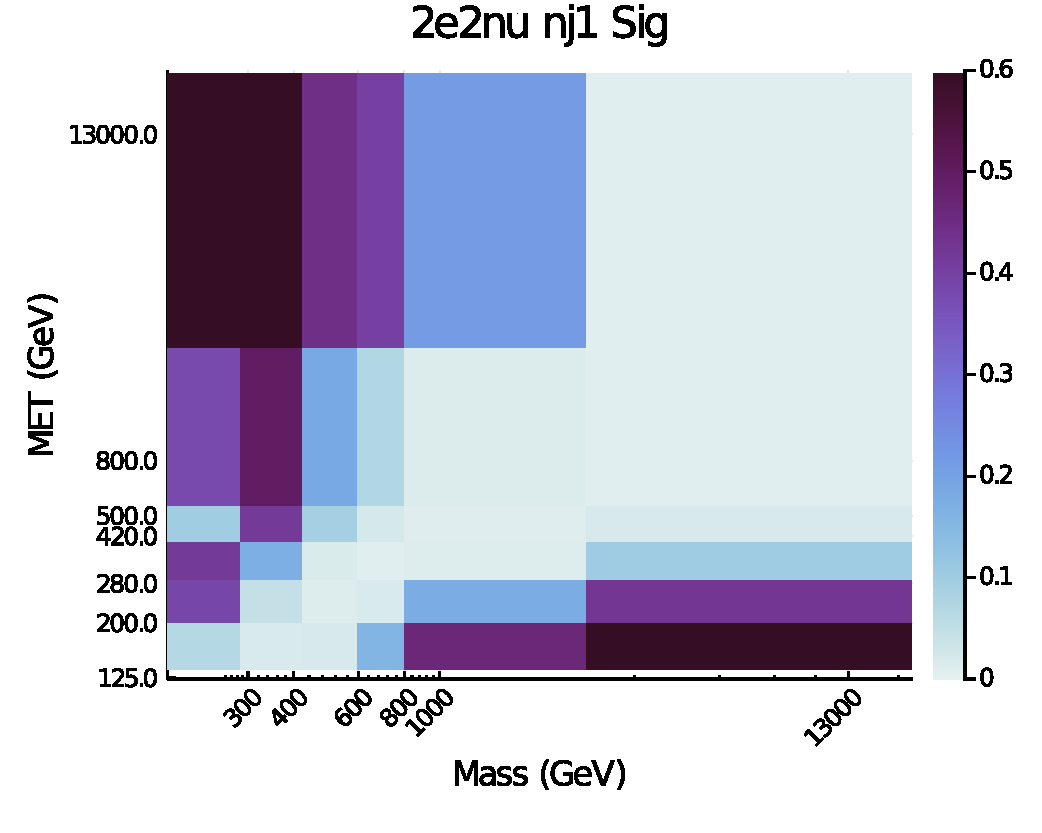
\includegraphics[width=.33\linewidth]{fig/ggZZ_templates/ggZZ_2e2nu_nj1_Sig.pdf}}
\subfloat[]{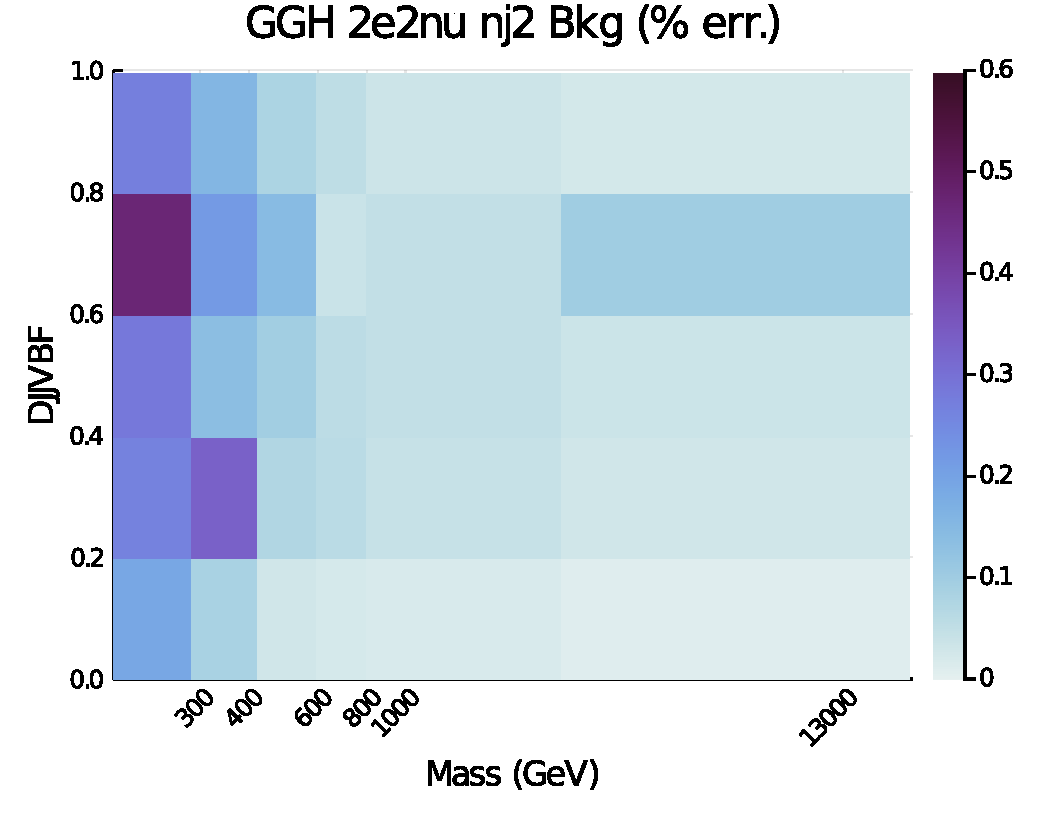
\includegraphics[width=.33\linewidth]{fig/ggZZ_templates/ggZZ_2e2nu_nj2_Bkg.pdf}}
\subfloat[]{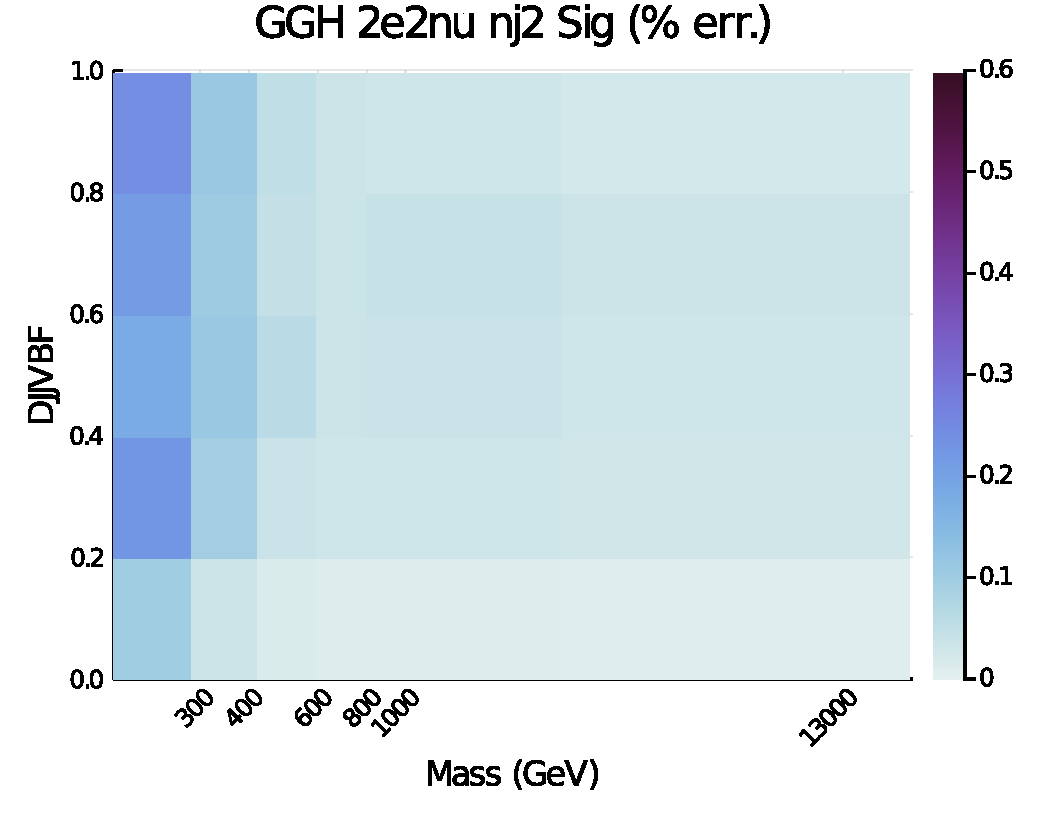
\includegraphics[width=.33\linewidth]{fig/ggZZ_templates/ggZZ_2e2nu_nj2_Sig.pdf}}\\
\subfloat[]{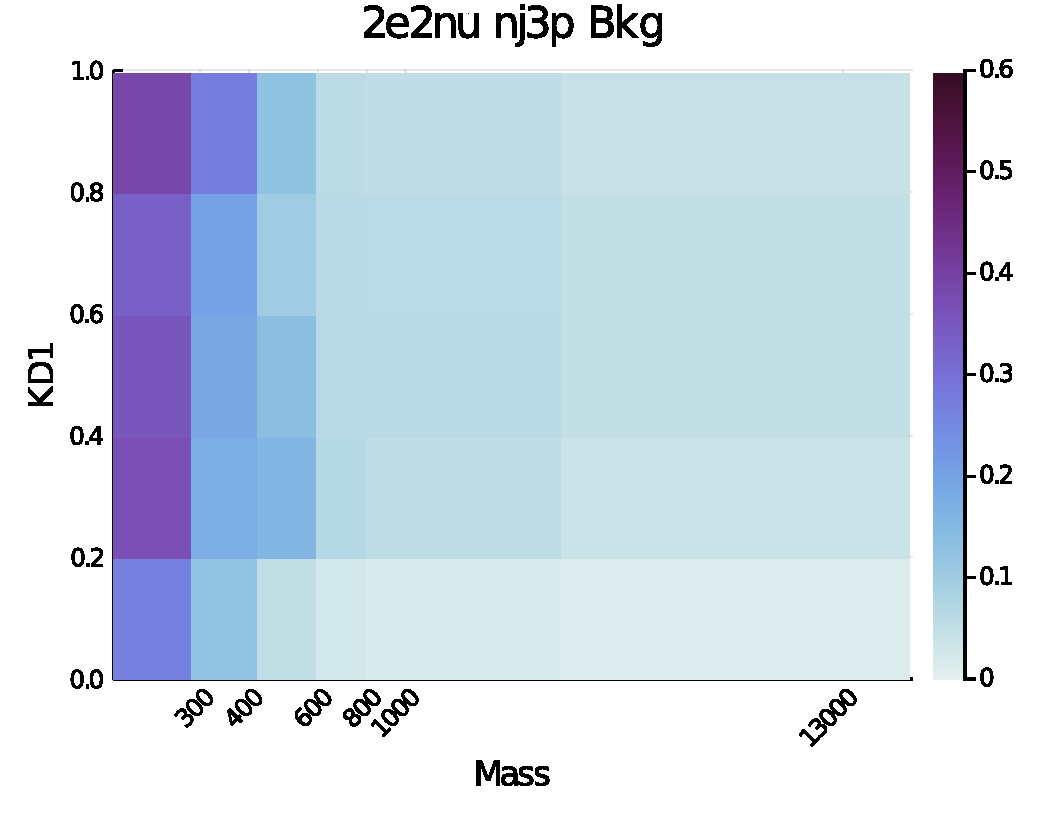
\includegraphics[width=.33\linewidth]{fig/ggZZ_templates/ggZZ_2e2nu_nj3p_Bkg.pdf}}
\subfloat[]{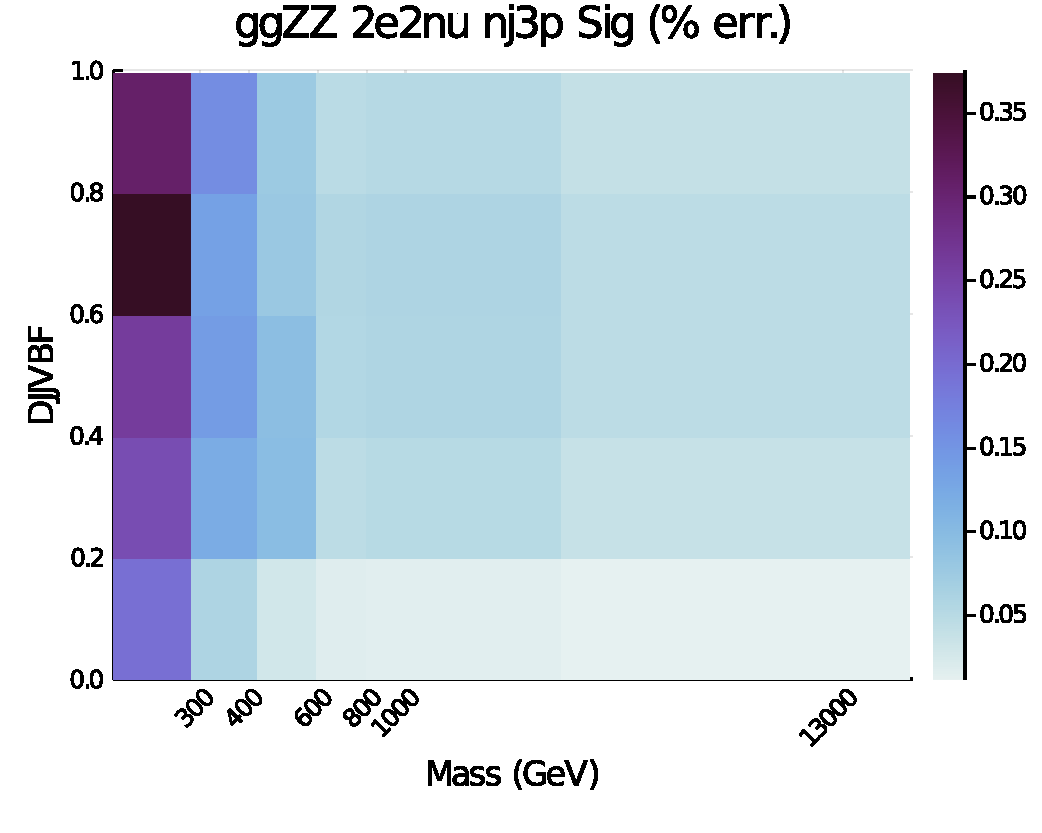
\includegraphics[width=.33\linewidth]{fig/ggZZ_templates/ggZZ_2e2nu_nj3p_Sig.pdf}}
\end{center}
\caption{Iterative sample mass factors obtained (left) and the final combined sample (right)}
\label{fig:LHE_rewgt}
\end{figure}

\begin{figure}[htb]
\begin{center}
\subfloat[]{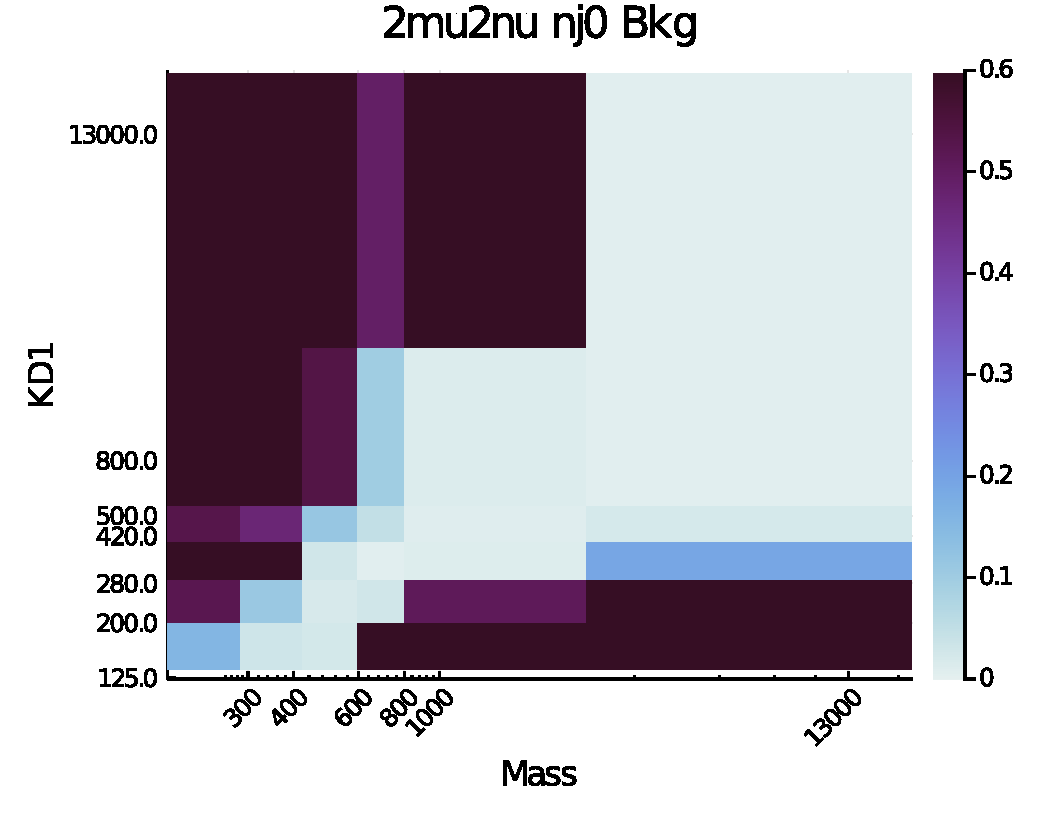
\includegraphics[width=.33\linewidth]{fig/ggZZ_templates/ggZZ_2mu2nu_nj0_Bkg.pdf}}
\subfloat[]{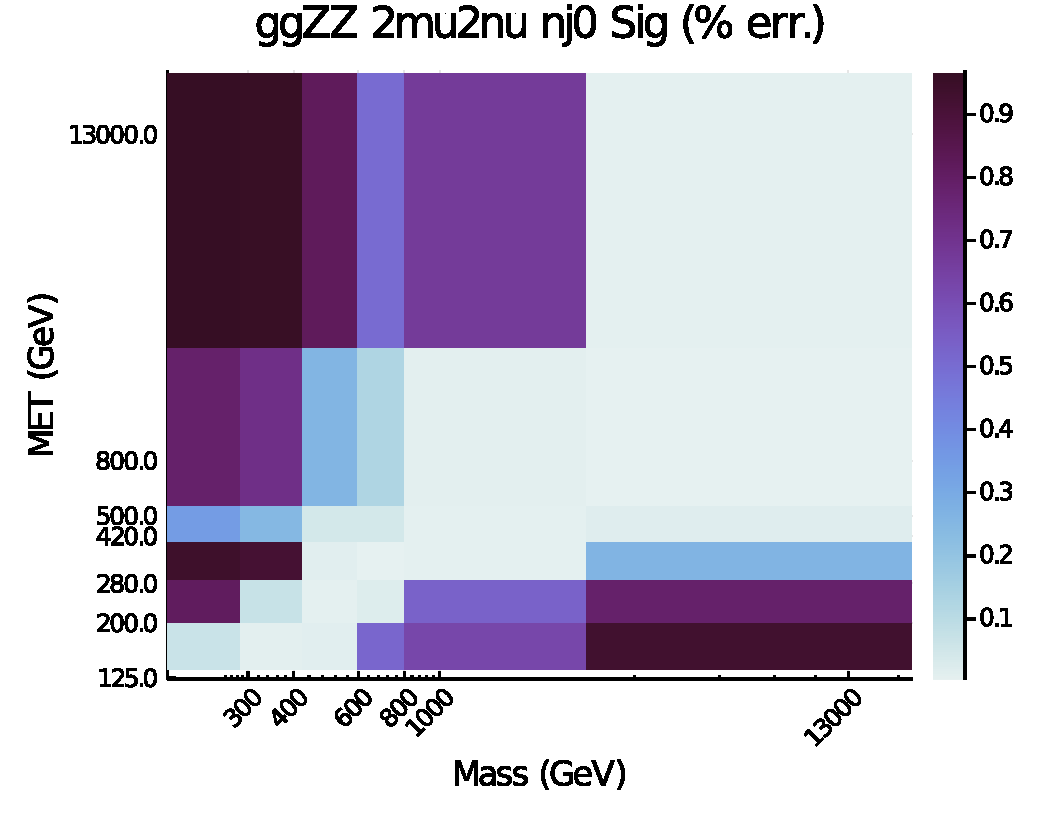
\includegraphics[width=.33\linewidth]{fig/ggZZ_templates/ggZZ_2mu2nu_nj0_Sig.pdf}}
\subfloat[]{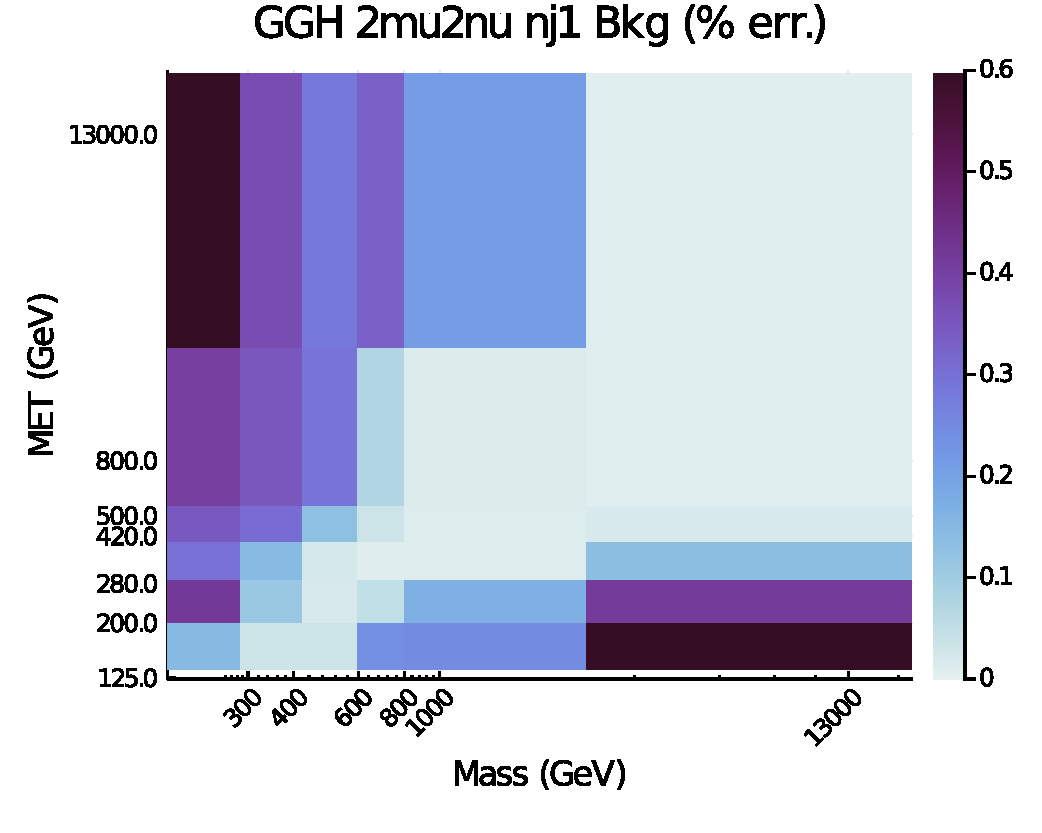
\includegraphics[width=.33\linewidth]{fig/ggZZ_templates/ggZZ_2mu2nu_nj1_Bkg.pdf}}\\
\subfloat[]{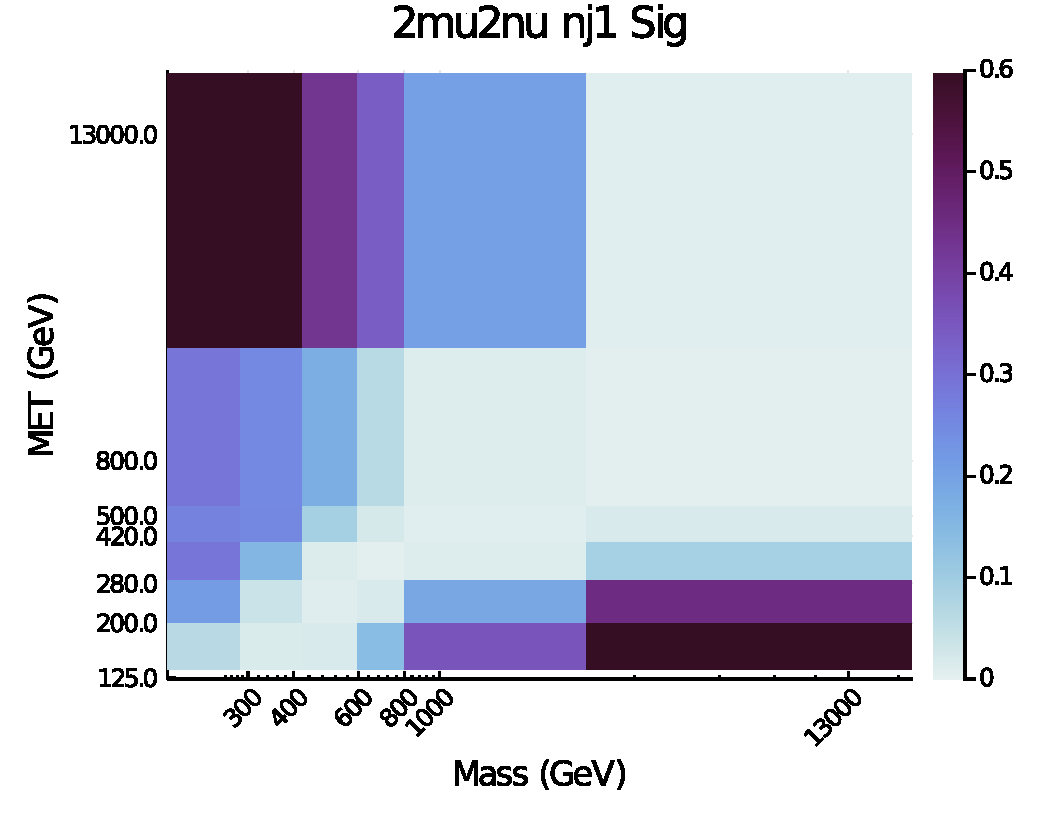
\includegraphics[width=.33\linewidth]{fig/ggZZ_templates/ggZZ_2mu2nu_nj1_Sig.pdf}}
\subfloat[]{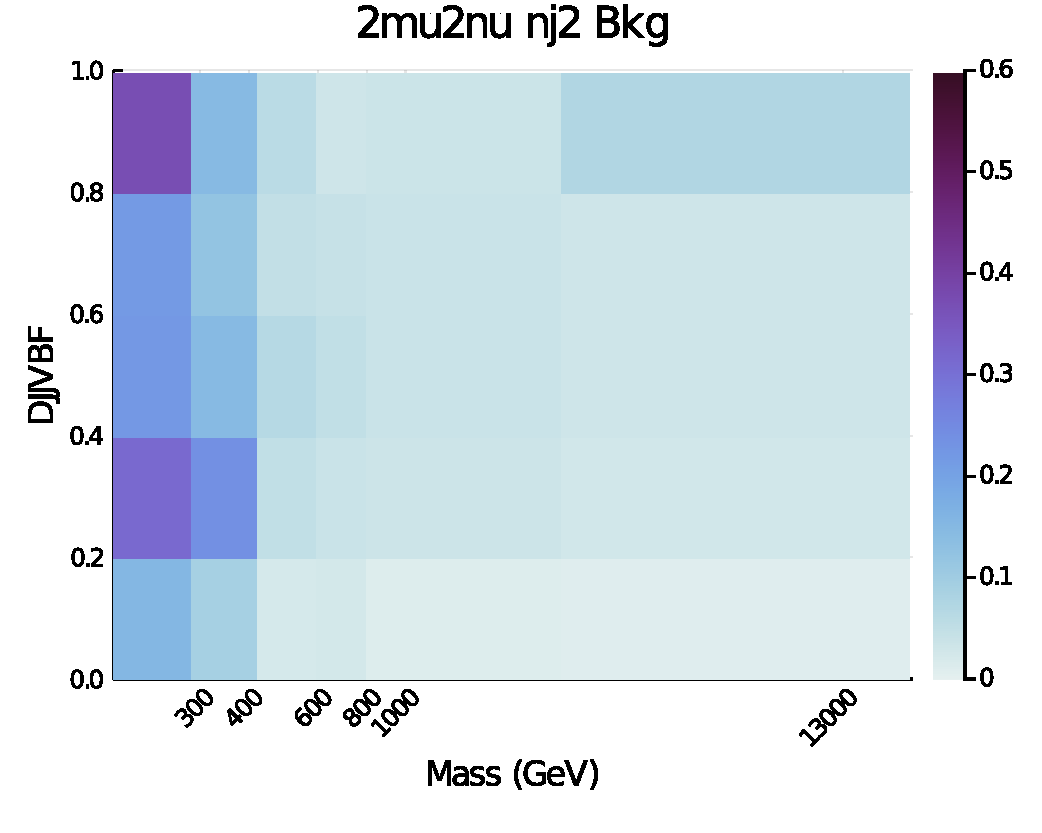
\includegraphics[width=.33\linewidth]{fig/ggZZ_templates/ggZZ_2mu2nu_nj2_Bkg.pdf}}
\subfloat[]{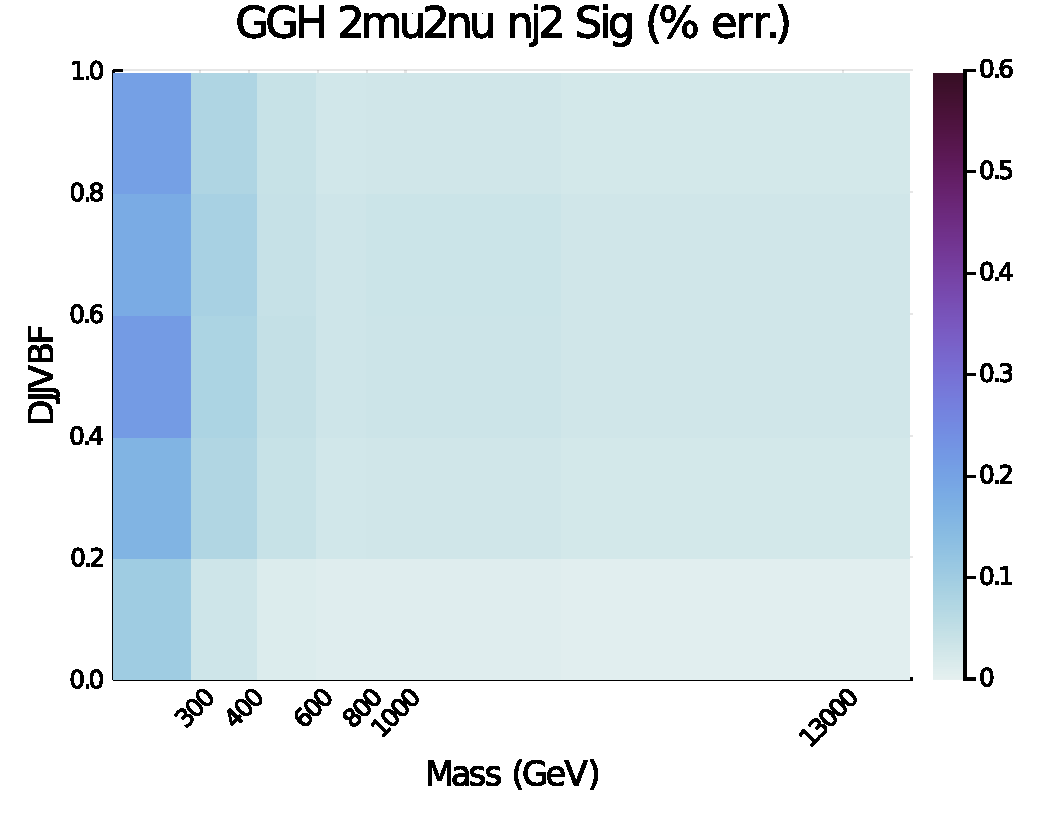
\includegraphics[width=.33\linewidth]{fig/ggZZ_templates/ggZZ_2mu2nu_nj2_Sig.pdf}}\\
\subfloat[]{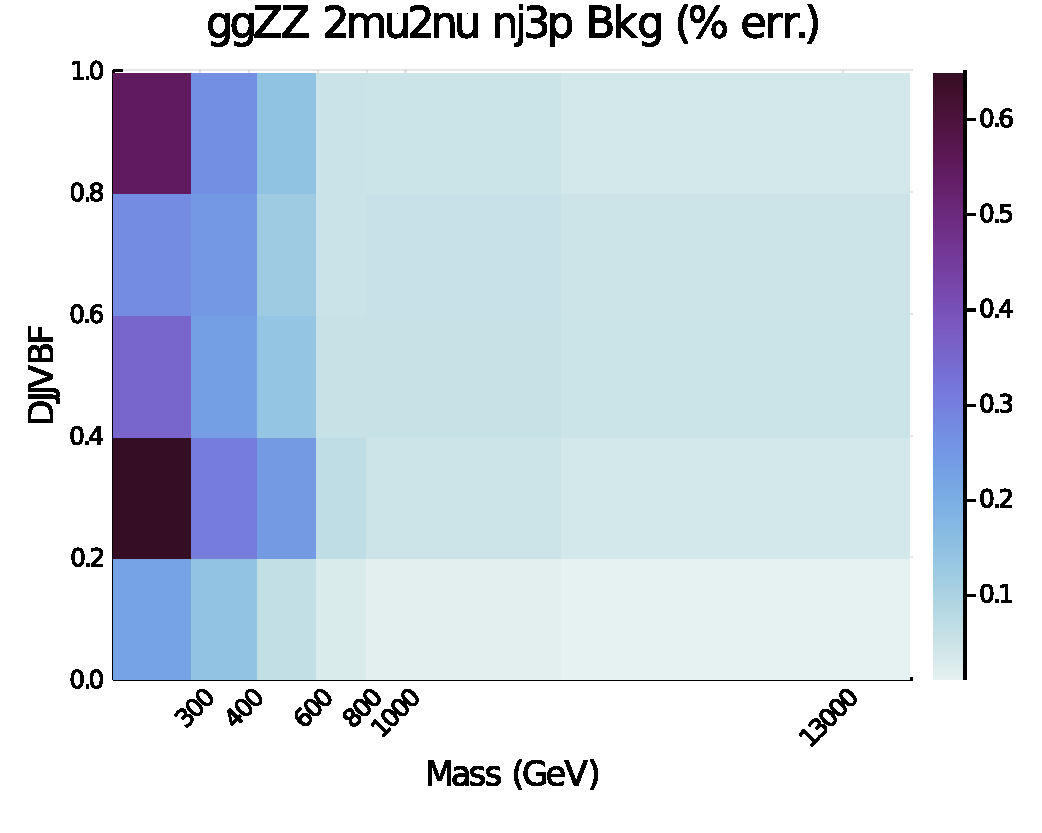
\includegraphics[width=.33\linewidth]{fig/ggZZ_templates/ggZZ_2mu2nu_nj3p_Bkg.pdf}}
\subfloat[]{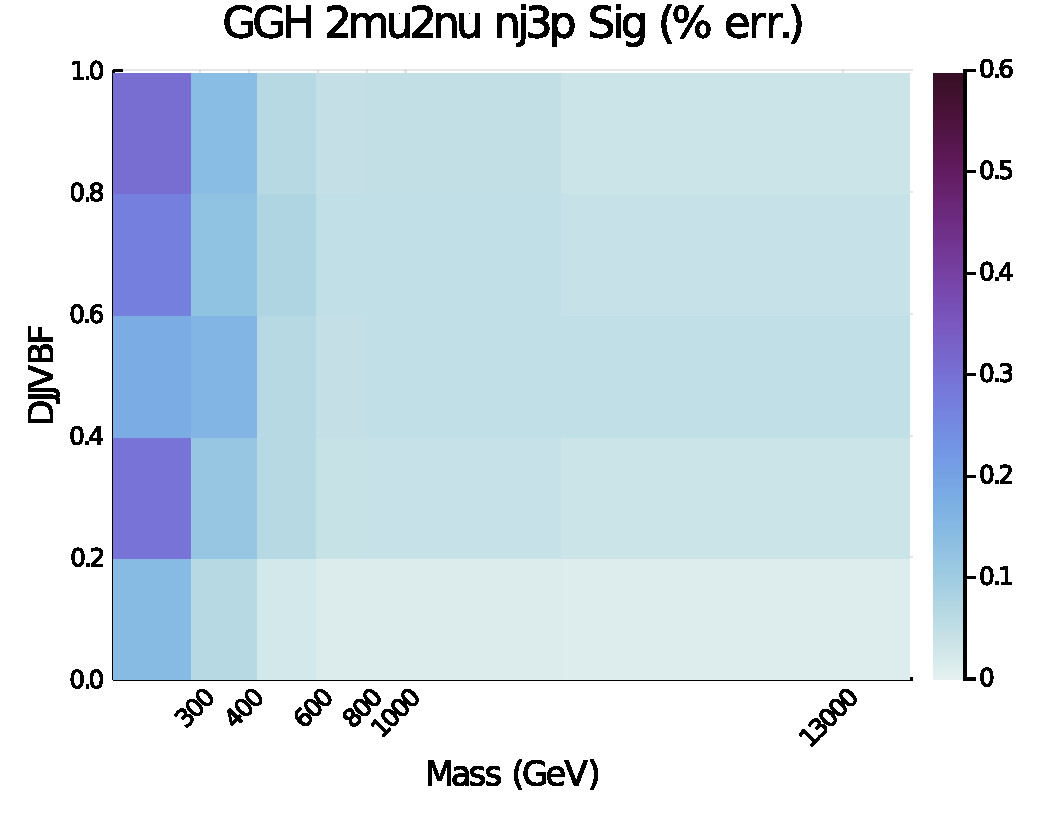
\includegraphics[width=.33\linewidth]{fig/ggZZ_templates/ggZZ_2mu2nu_nj3p_Sig.pdf}}
\end{center}
\caption{Iterative sample mass factors obtained (left) and the final combined sample (right)}
\label{fig:LHE_rewgt}
\end{figure}


\end{mainmatter}
\ssp
\bibliographystyle{JHEP3}
\bibliography{dissertation}
\end{document}
